The client application was built around the framework Next.js (not to be confused with NestJS, a different framework, used in the implementation of previously described services). Next.js~\cite{next_js} \enquote{is a React framework for building full-stack web applications.} \enquote{Under the hood, Next.js also abstracts and automatically configures tooling needed for React, like bundling, compiling, and more.} Some of its main features include:
\begin{itemize}
    \item \textbf{Routing} --- \enquote{A file-system based router built on top of Server Components that supports layouts, nested routing, loading states, error handling, and more.}
    \item \textbf{Rendering} --- \enquote{Client-side and Server-side Rendering with Client and Server Components. Further optimized with Static and Dynamic Rendering on the server with Next.js. Streaming on Edge and Node.js runtimes.}
    \item \textbf{Data Fetching} --- \enquote{Simplified data fetching with async/await in Server Components, and an extended \mintinline{ts}{fetch} API for request memoization, data caching and revalidation.}
    \item \textbf{Styling} --- \enquote{Support for your preferred styling methods, including CSS Modules, Tailwind CSS, and CSS-in-JS.}
    \item \textbf{Optimizations} --- \enquote{Image, Fonts, and Script Optimizations to improve your application's Core Web Vitals and User Experience.}
    \item \textbf{TypeScript} --- \enquote{Improved support for TypeScript, with better type checking and more efficient compilation, as well as custom TypeScript Plugin and type checker.}
\end{itemize}

The MaterialUI component library was used during the creation of the pages.

\subsection{Pages}

\fboxsep=0pt

\subsubsection{Authentication}

When a user accesses any part of the client application without being signed into an account, they are redirected to the authentication page, available under the path \mintinline{text}{/auth}. This redirection and validation of user sessions is handled by the \mintinline{ts}{SuperTokensWrapper} and \mintinline{ts}{SessionAuth} components from the SuperTokens SDK, which surround the contents of a page that requires authentication (in this case all pages).

The authentication page can be seen in the figure~\ref{fig:auth_page} and contains another component from the SuperTokens SDK, that is configured based on the desired authentication methods. The methods chosen are email with password, and third-party social login using a GitHub account. The component features a button for the social sign-in alongside two input fields and a confirmation button for the email with password sign-in method. The default state for the component is sign in (log in with an existing account). This state can be changed to sign up (create a new account) with a button present at the top of the component. Furthermore, there is also a \enquote{forgot password} button which, upon activation, switches the component to another state where the user inputs their account email address and confirms that they wish to reset their password. The user is then sent an email with a password reset link which, when opened, allows the user to choose their new password.

\begin{figure}
    \centering
    \fbox{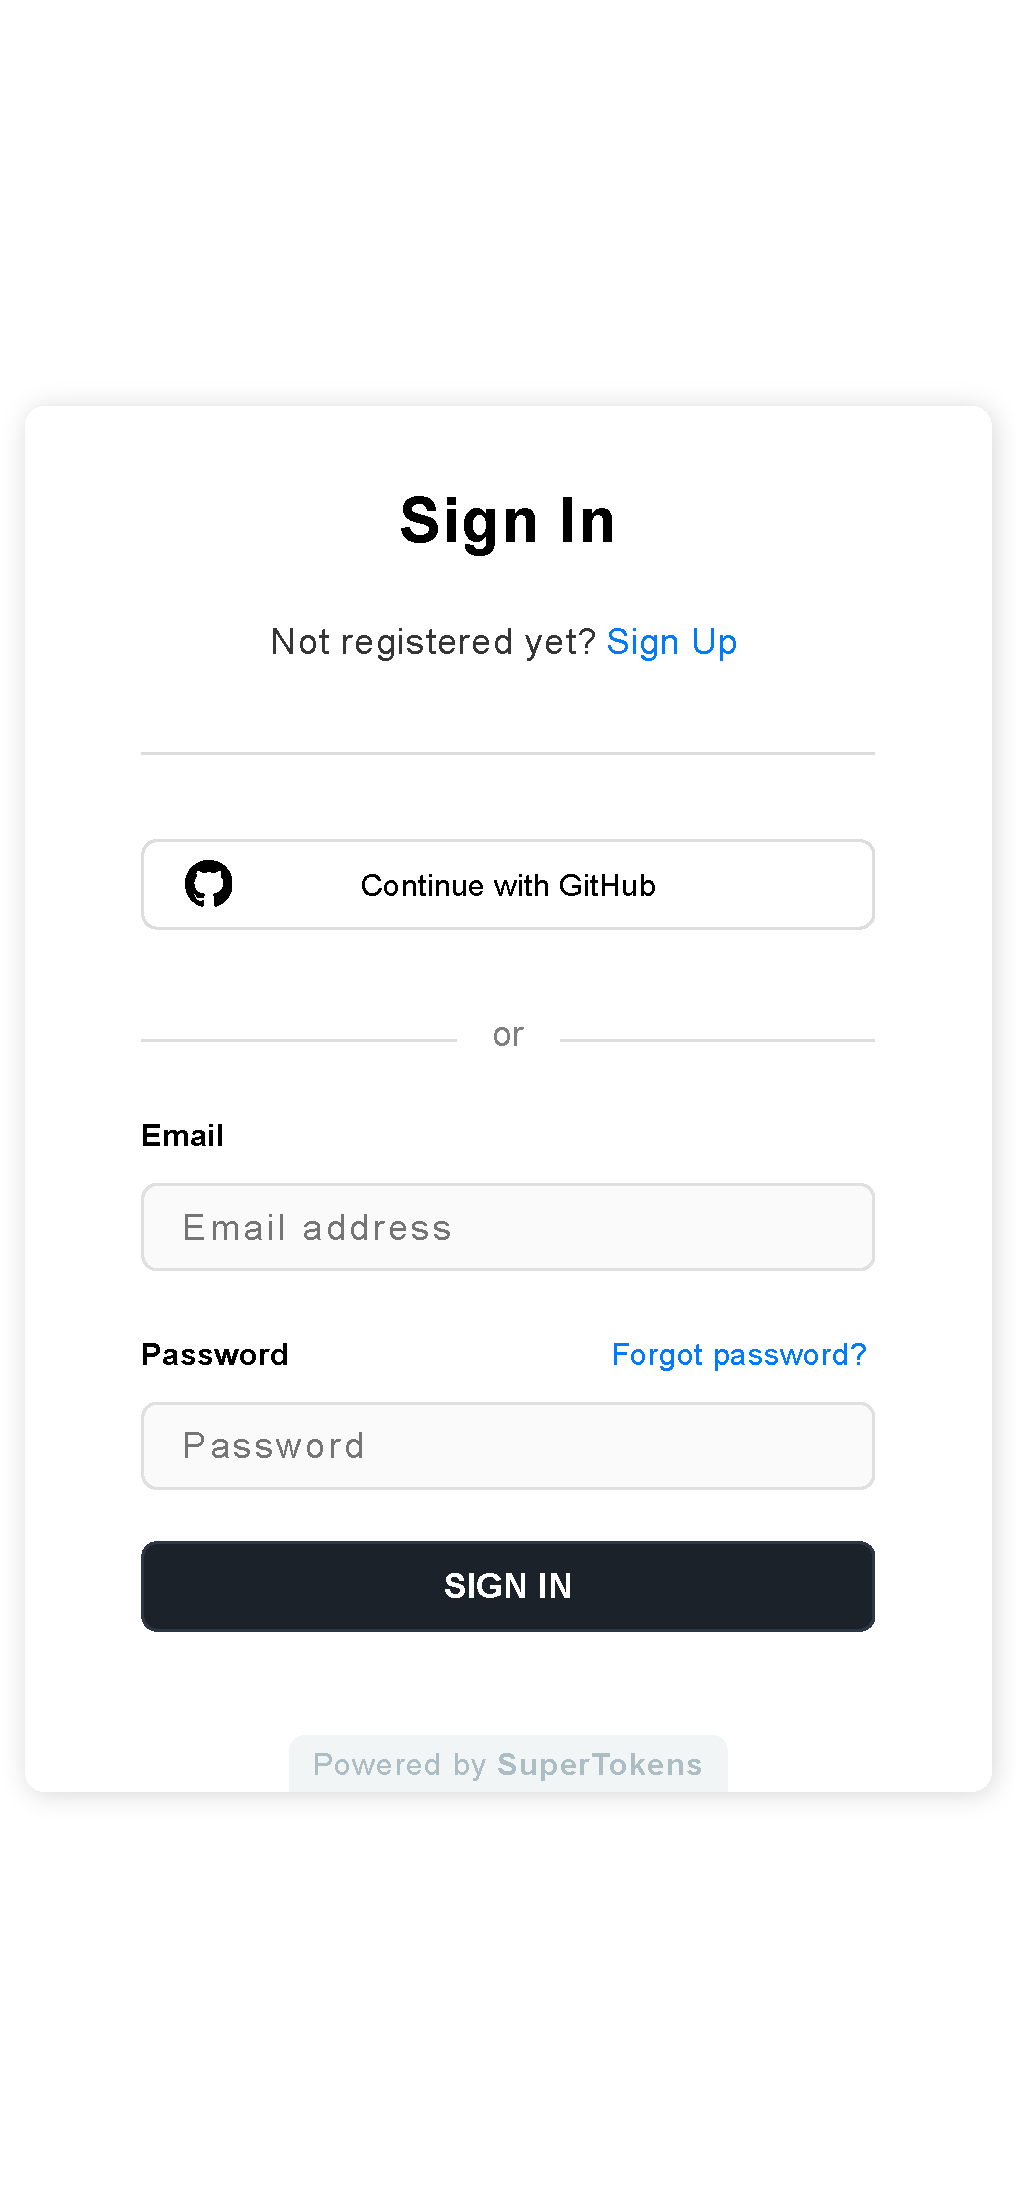
\includegraphics[width=0.48\textwidth]{content/implementation/client_app_auth_sign_in.pdf}}
    \hfill
    \fbox{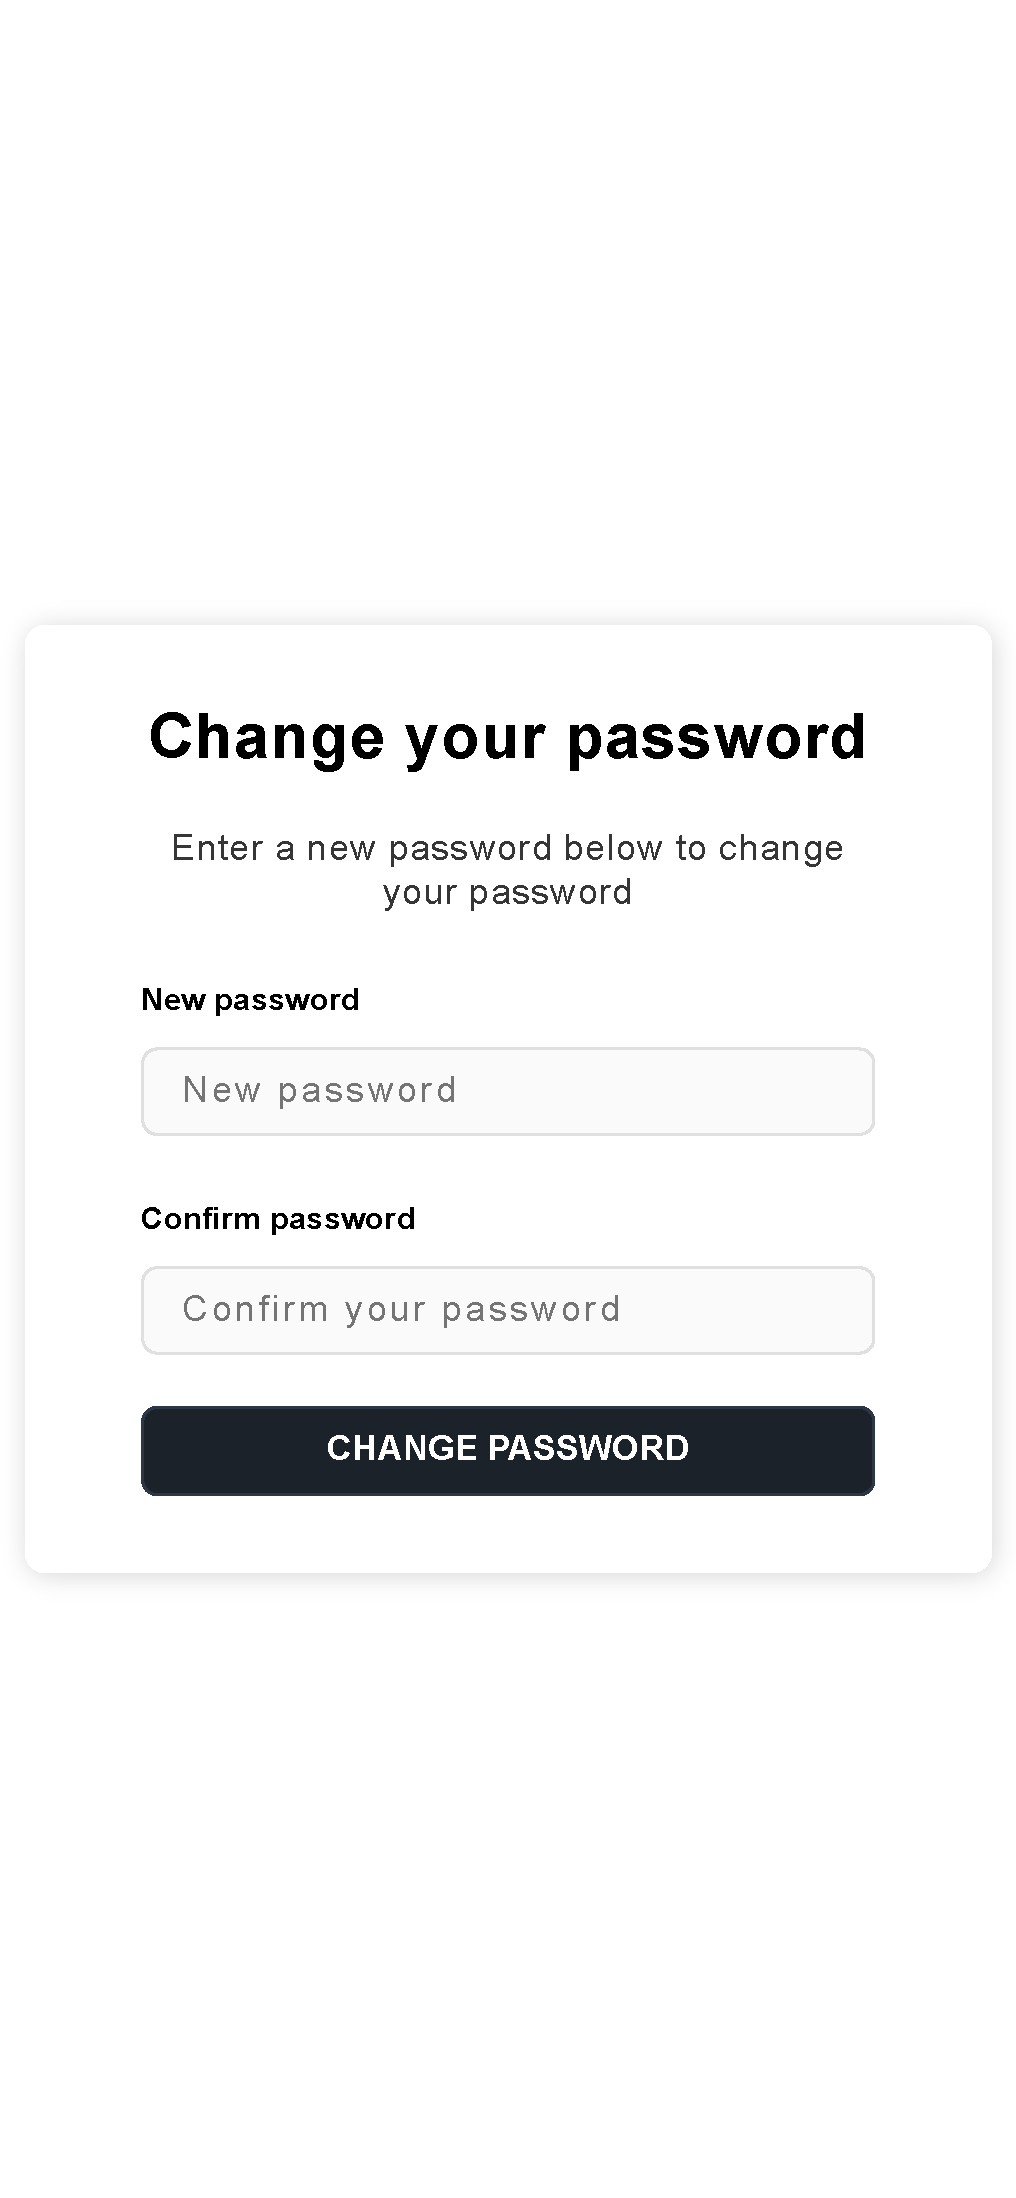
\includegraphics[width=0.48\textwidth]{content/implementation/client_app_auth_password_reset_change.pdf}}
    \caption[Authentication page]{Authentication page with a SuperTokens component in the sign-in state seen left, password reset seen right.}
    \label{fig:auth_page}
\end{figure}

\subsubsection{Home}

The home page, available under the path \mintinline{text}{/}, is divided into three main states: booking address creation, an overview of user's bookings, and an item booking detail.

If the user has not yet created a booking address, they are prompted to do so. The page then contains a one-field form, where the user fills in their desired booking address username. This username, along with the booking service provider's provided hostname, then forms the user's new booking address. During the process of choosing their username, the user gets immediate feedback if the username is invalid. The user then confirms their username selection, upon which either their new booking address is created, moving them to the home page state with an overview of their bookings or, if their booking address was already used by another user, an alert is displayed with an informative error (the alert can be hidden by clicking on it). The username input and validation can be seen in the figure~\ref{fig:home_page_create_address_1}, while the confirmation and error can be seen in the figure~\ref{fig:home_page_create_address_2}. This, along with the authentication page, fulfills functional requirement~\ref{req:user_account}.

\begin{figure}
    \centering
    \fbox{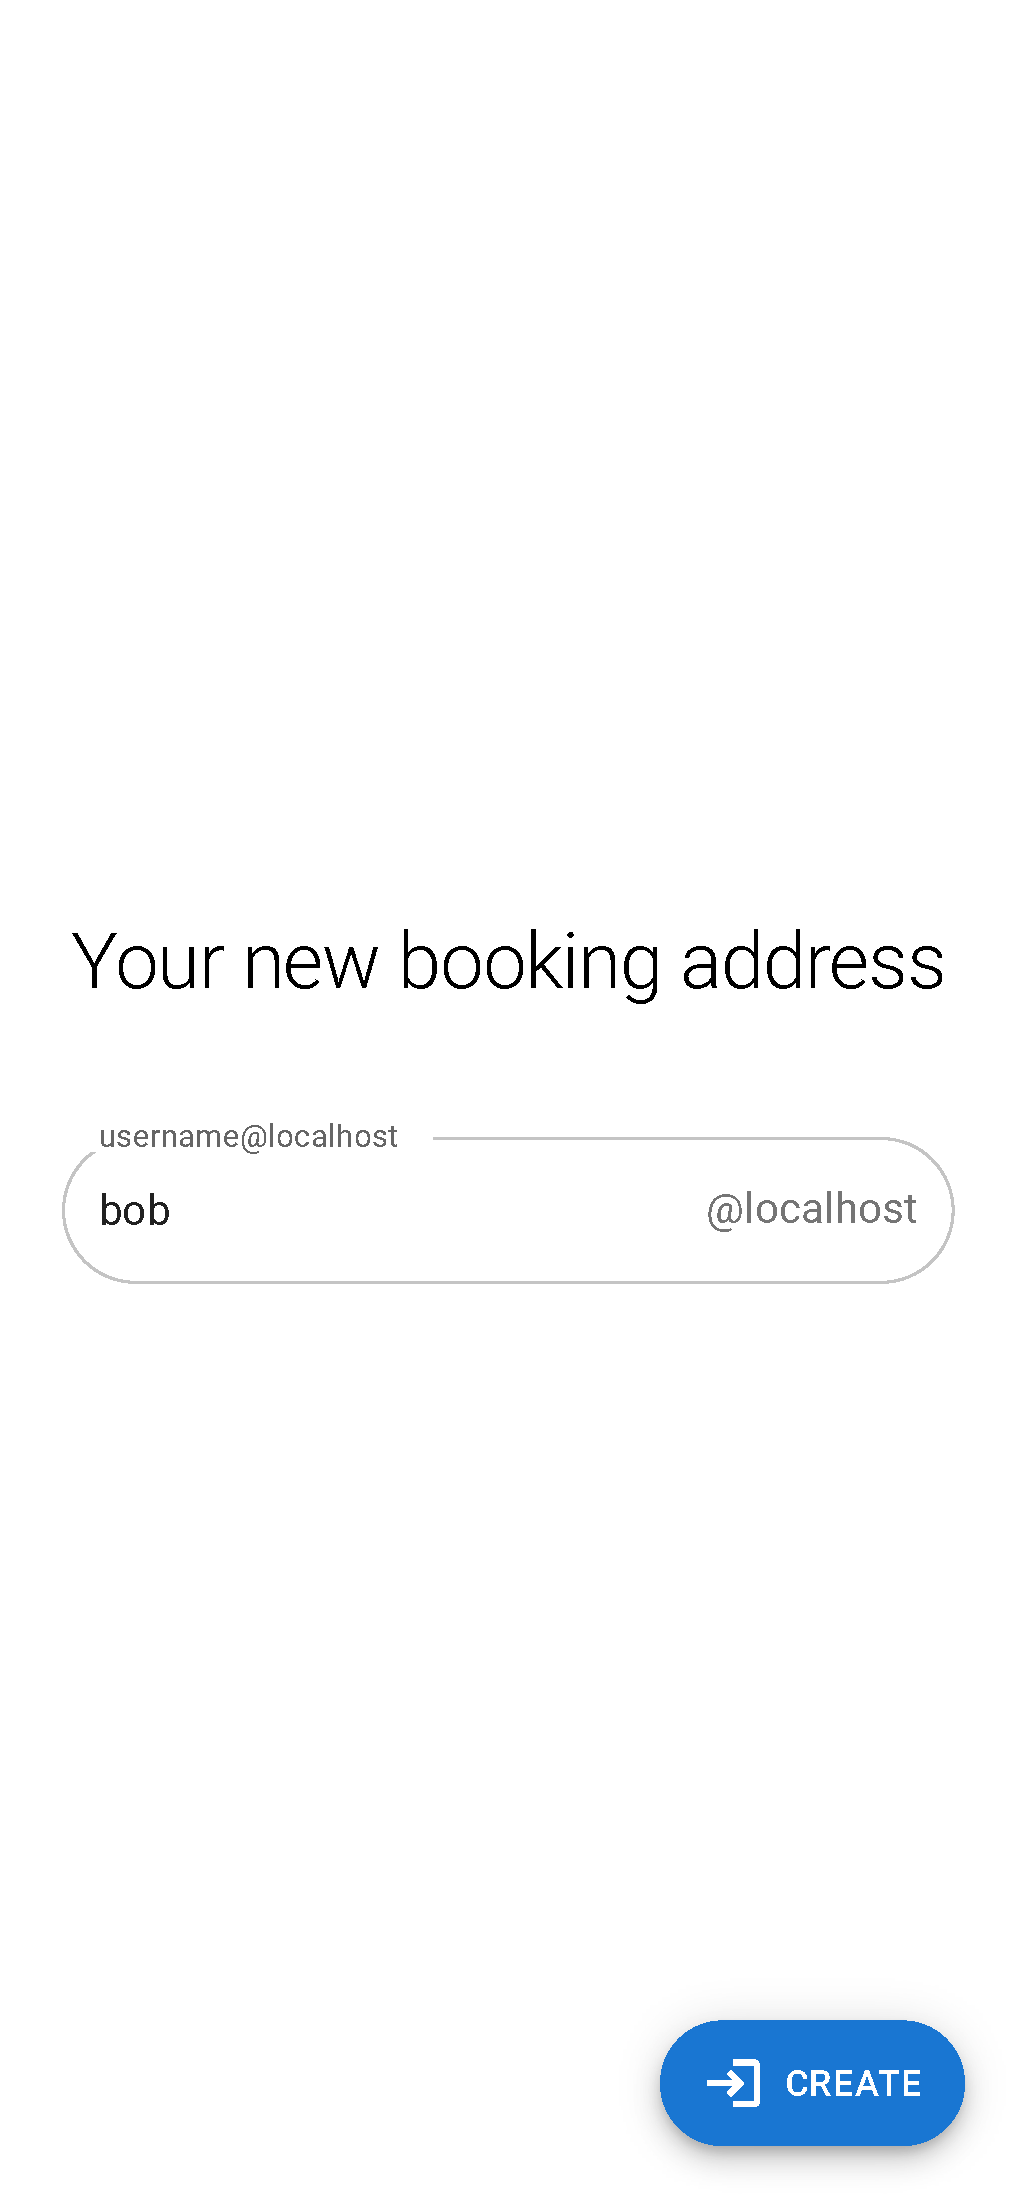
\includegraphics[width=0.48\textwidth]{content/implementation/client_app_create_address_filled.pdf}}
    \hfill
    \fbox{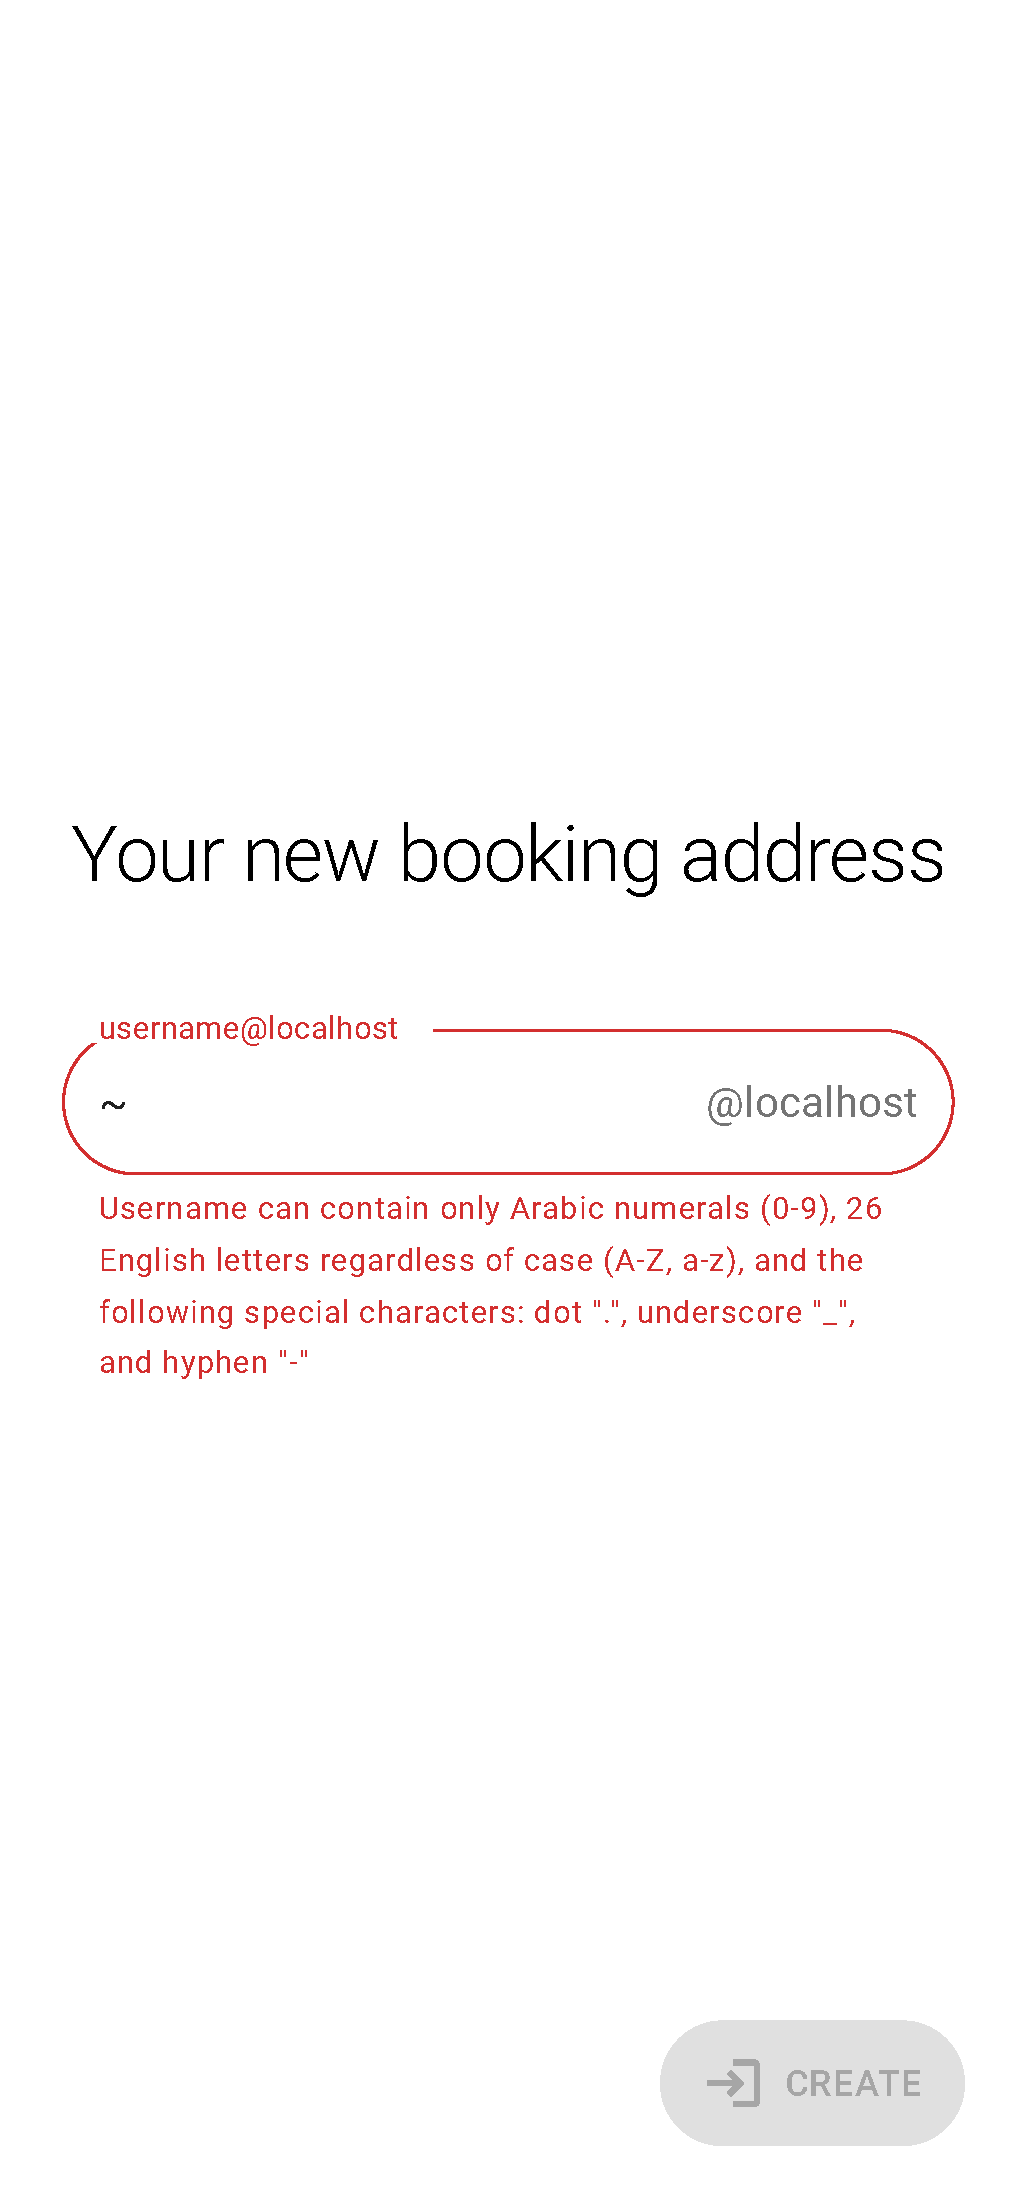
\includegraphics[width=0.48\textwidth]{content/implementation/client_app_create_address_invalid.pdf}}
    \caption[Home page -- Creation of booking address: input and validation]{Home page in the create booking address state with booking address username input seen left and its validation to the right}
    \label{fig:home_page_create_address_1}
\end{figure}

\begin{figure}
    \centering
    \fbox{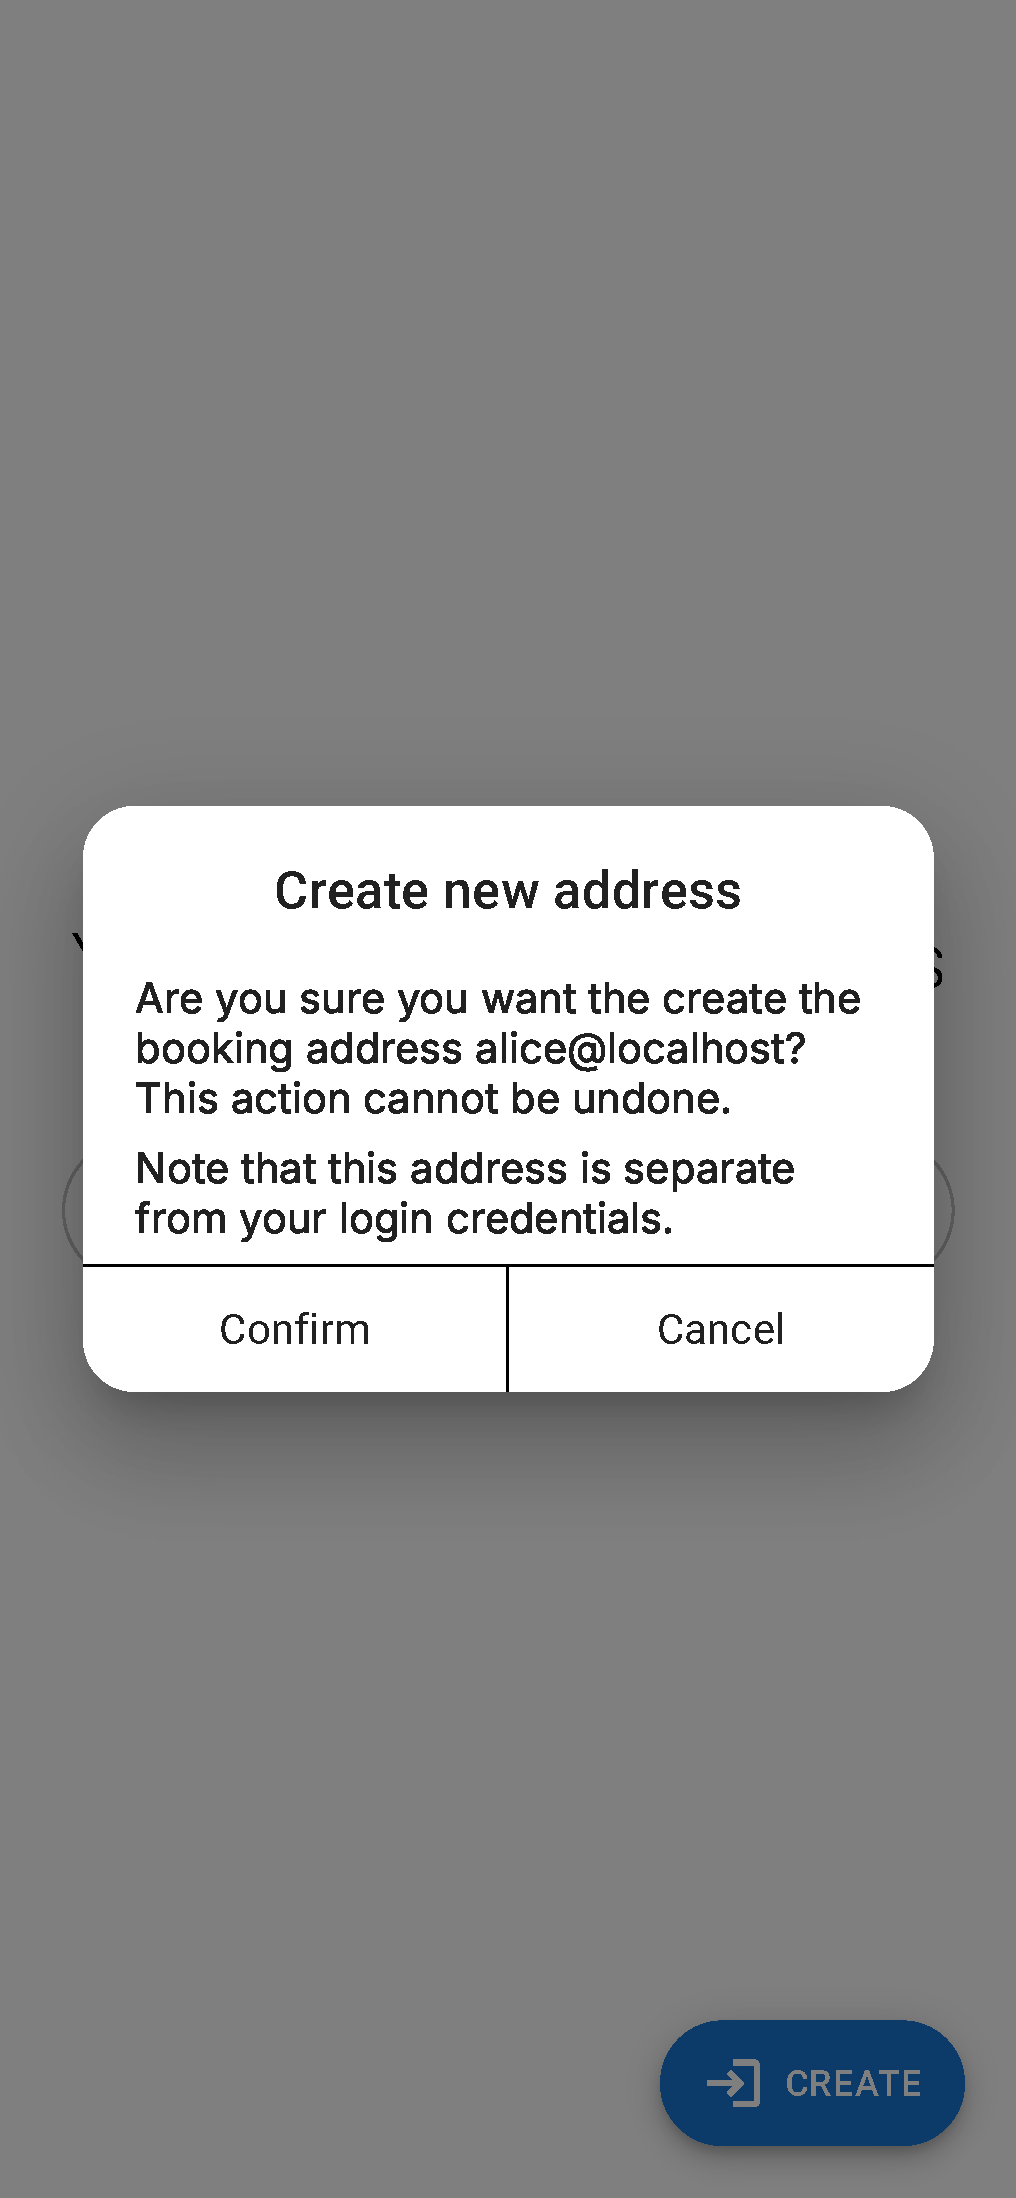
\includegraphics[width=0.48\textwidth]{content/implementation/client_app_create_confirm.pdf}}
    \hfill
    \fbox{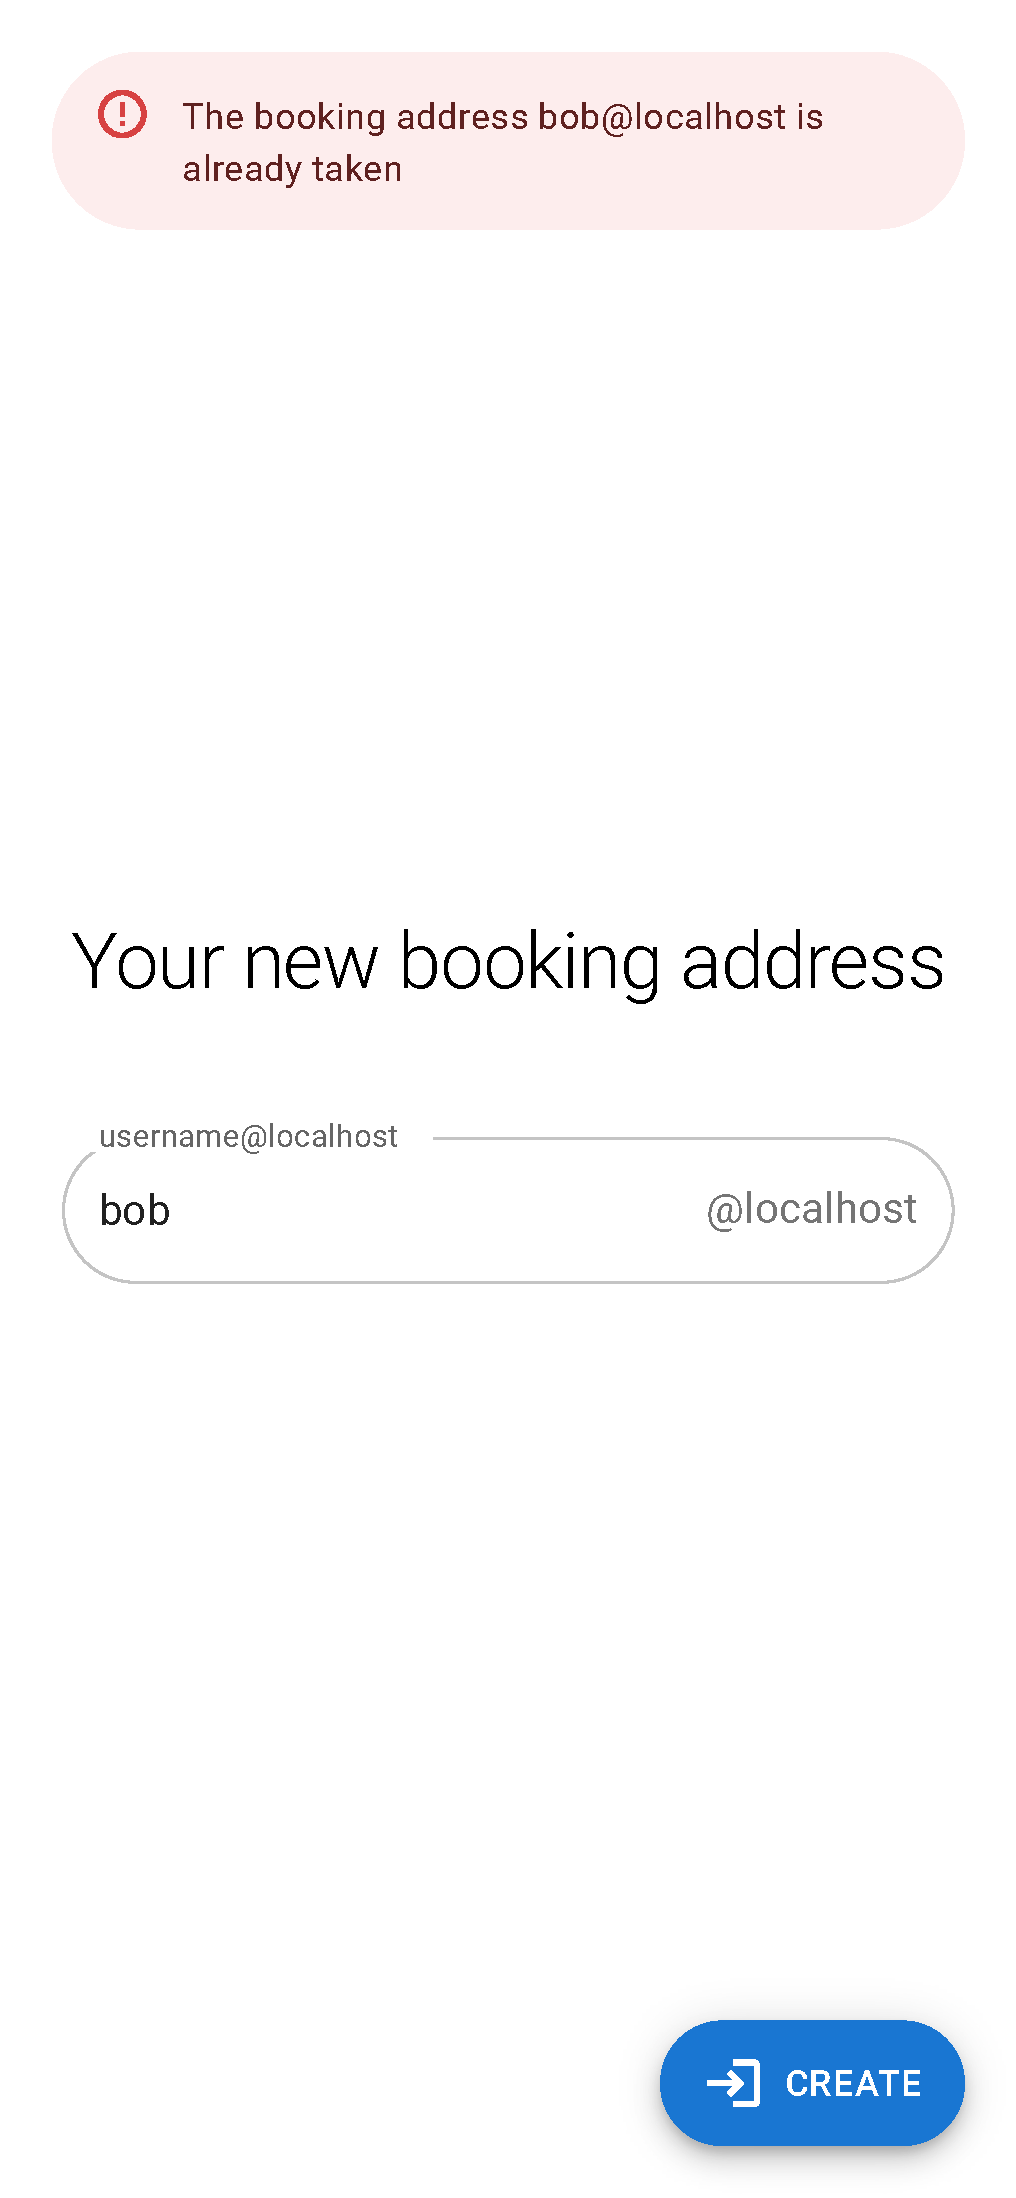
\includegraphics[width=0.48\textwidth]{content/implementation/client_app_create_address_error.pdf}}
    \caption[Home page -- Creation of booking address: confirmation and error]{Home page in the create booking address state with confirmation before address creation seen left and an error due to the address being taken seen to the right}
    \label{fig:home_page_create_address_2}
\end{figure}

The overview of user's bookings contains a vertical list of the items, that the user has booked. This overview can be seen in the figure~\ref{fig:home_page_bookings} Each item lists the inventory owner's booking address at the top, and item metadata at the bottom, as many as can fit onto one line. Upon clicking an item from the list, the user is moved to the third state of the home page, the item booking detail. A menubar is present at the top of the bookings list, with a \enquote{burger} button that opens a drawer with links to the main client application sections (the currently active home page, and the business page), a search bar for searching within the bookings (currently not implemented), and a button with a profile icon that opens a dialog with the user's booking address and a log out button. The open drawer and profile dialog are displayed in the figure~\ref{fig:home_page_bookings_drawer_profile}. To the bottom-right corner of the page, a \enquote{book} button is present, that redirects the user to the new booking page.

\begin{figure}
    \centering
    \fbox{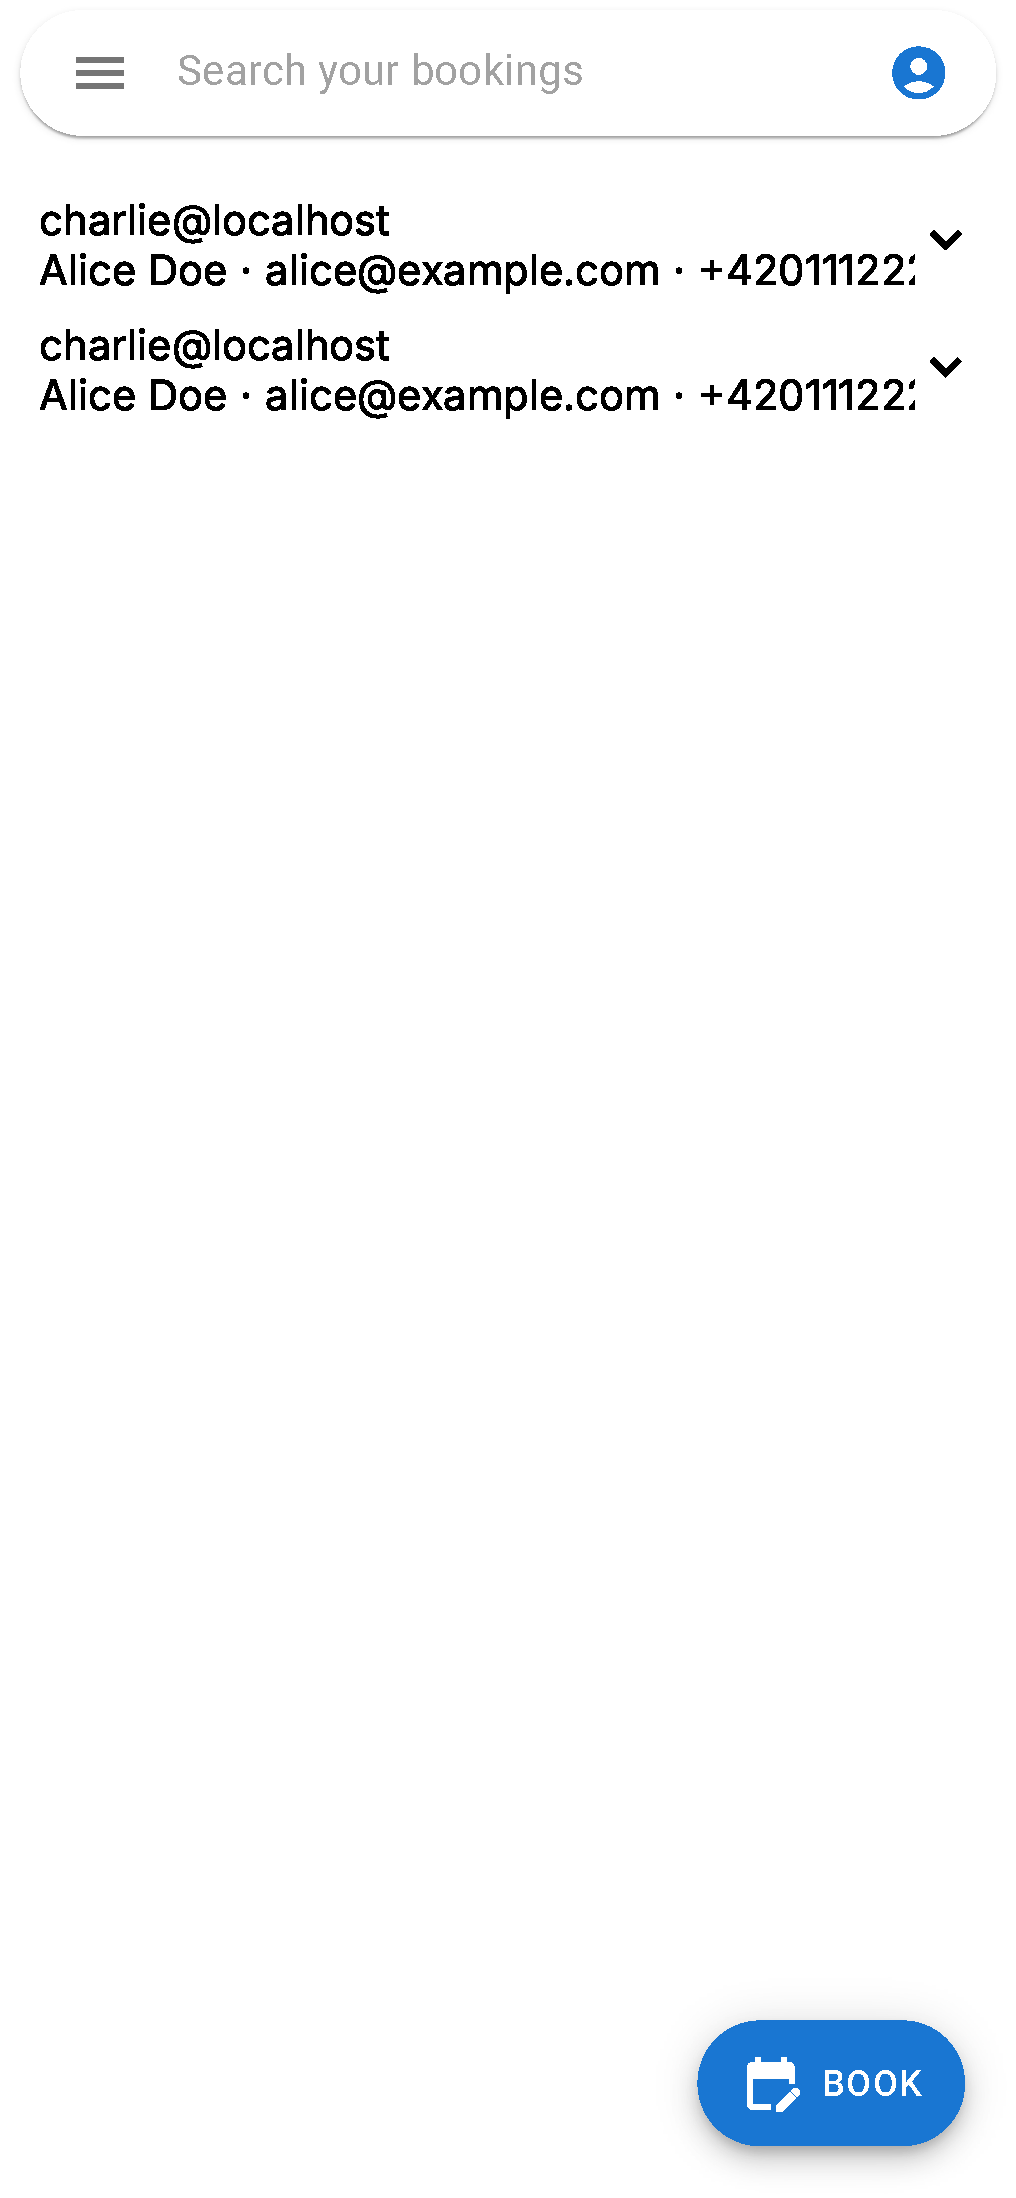
\includegraphics[width=0.48\textwidth]{content/implementation/client_app_home_bookings.pdf}}
    \caption[Home page -- Bookings overview]{Home page in the bookings overview state}
    \label{fig:home_page_bookings}
\end{figure}

\begin{figure}
    \centering
    \fbox{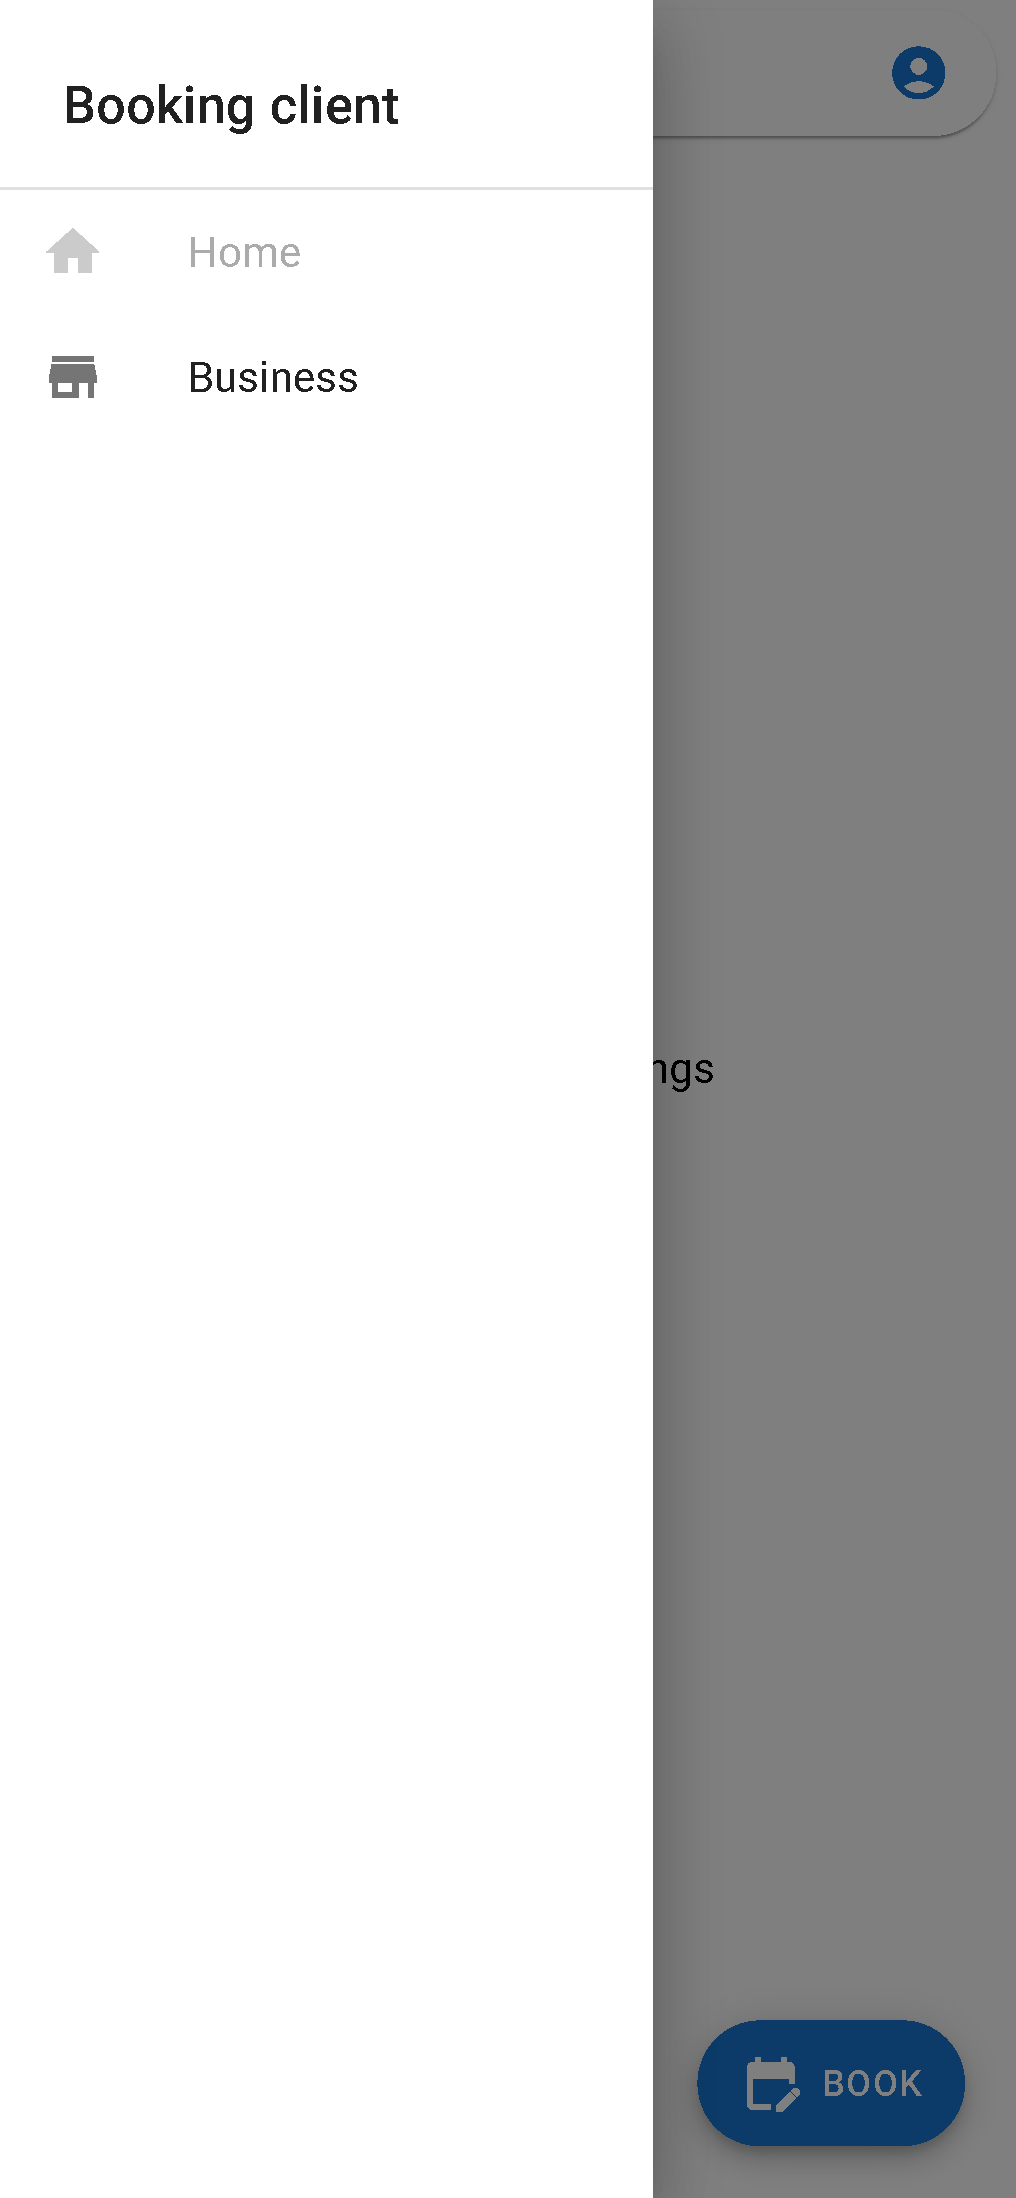
\includegraphics[width=0.48\textwidth]{content/implementation/client_app_home_drawer.pdf}}
    \hfill
    \fbox{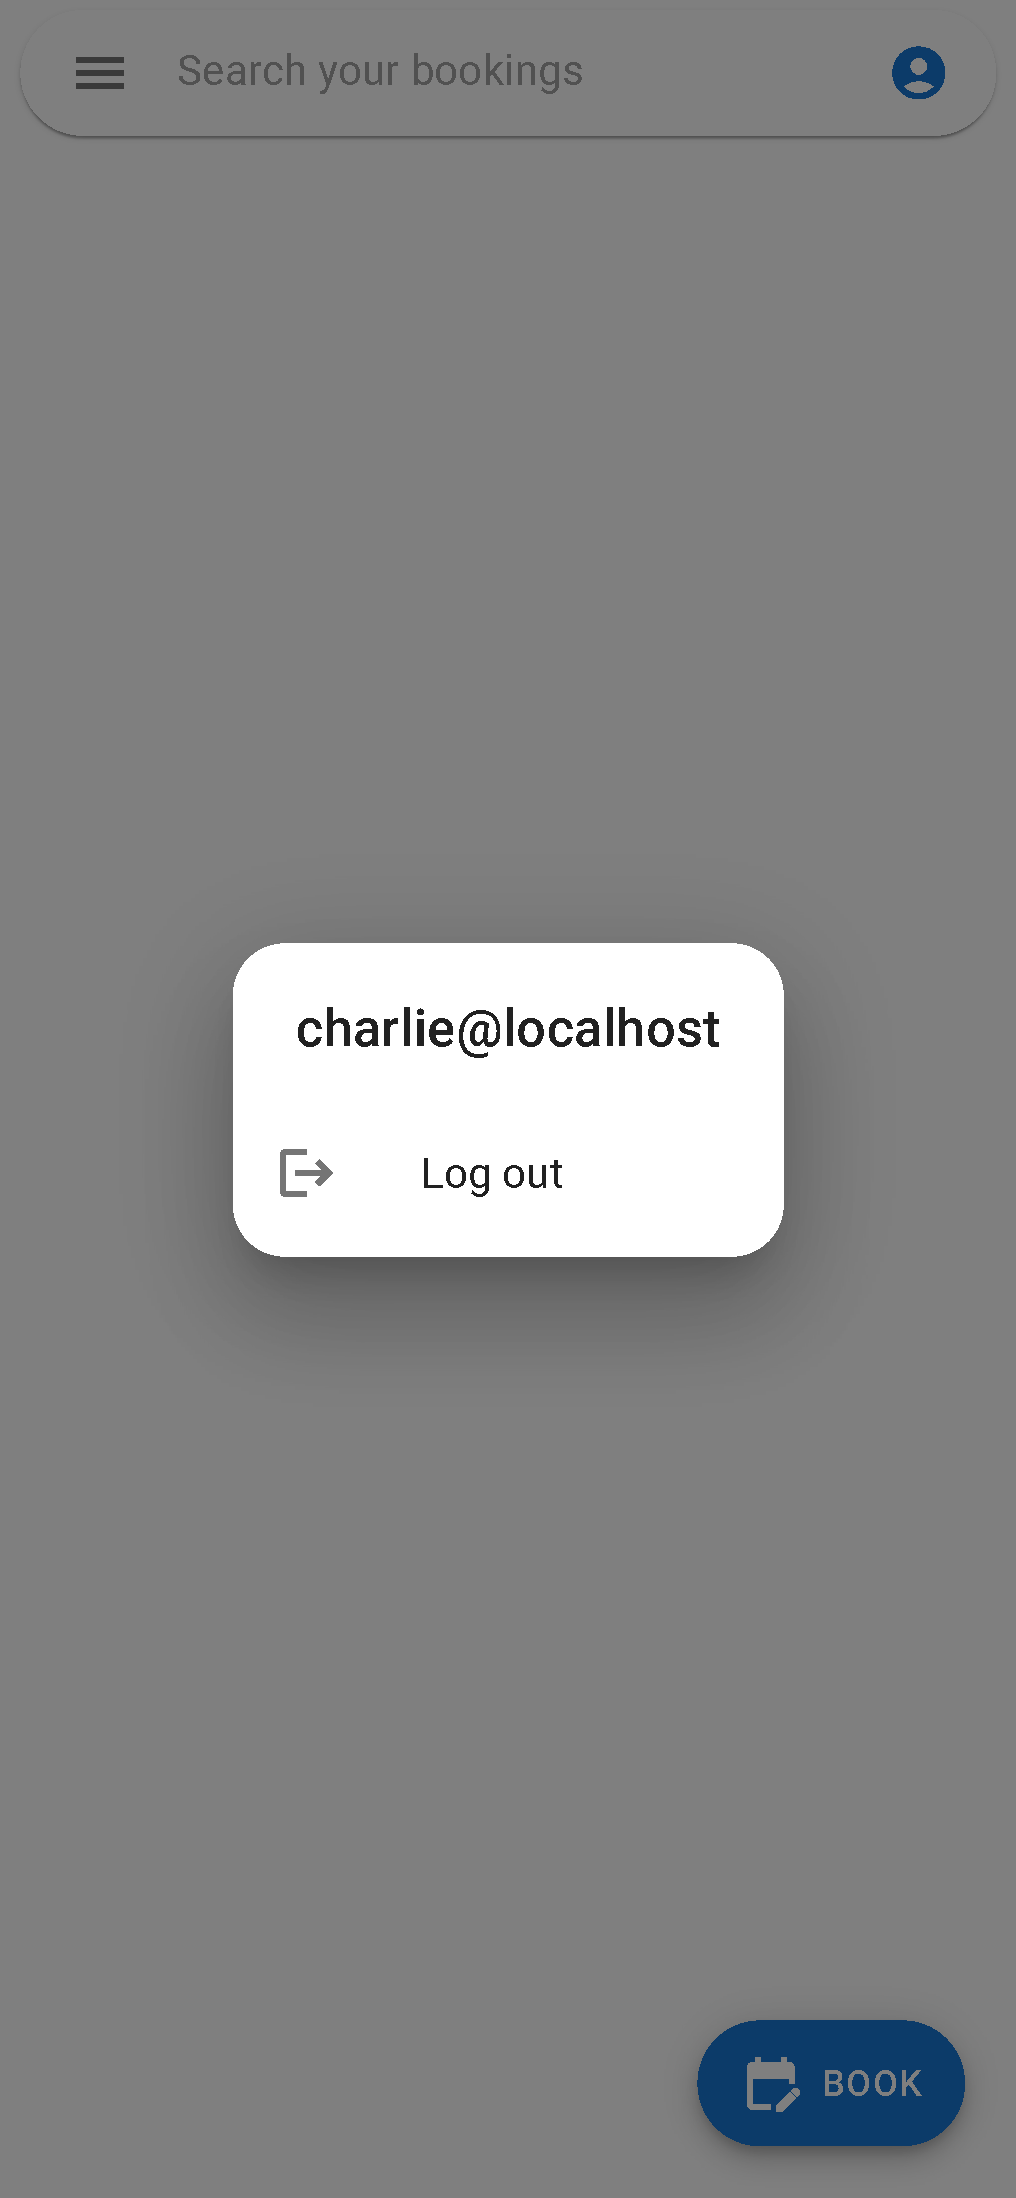
\includegraphics[width=0.48\textwidth]{content/implementation/client_app_home_profile.pdf}}
    \caption[Home page -- Open drawer and profile dialog]{Open drawer with main website section links seen left, dialog with profile information and log out button seen right}
    \label{fig:home_page_bookings_drawer_profile}
\end{figure}

The item booking detail, which is shown in the figure~\ref{fig:home_page_booking_details}, contains a list of information about the booked item, including its inventory's owner's booking address and the item's metadata. This list is followed by listed form data, that the user filled in during booking. At the top, there is a title of the page state along with a back button that allows the user to move back to the bookings overview state.

The reason for keeping the item booking detail a state of the home page, instead of its own separate page, is that the home page already has all the data needed, therefore preventing unnecessary data fetching from the booking service.

\begin{figure}
    \centering
    \fbox{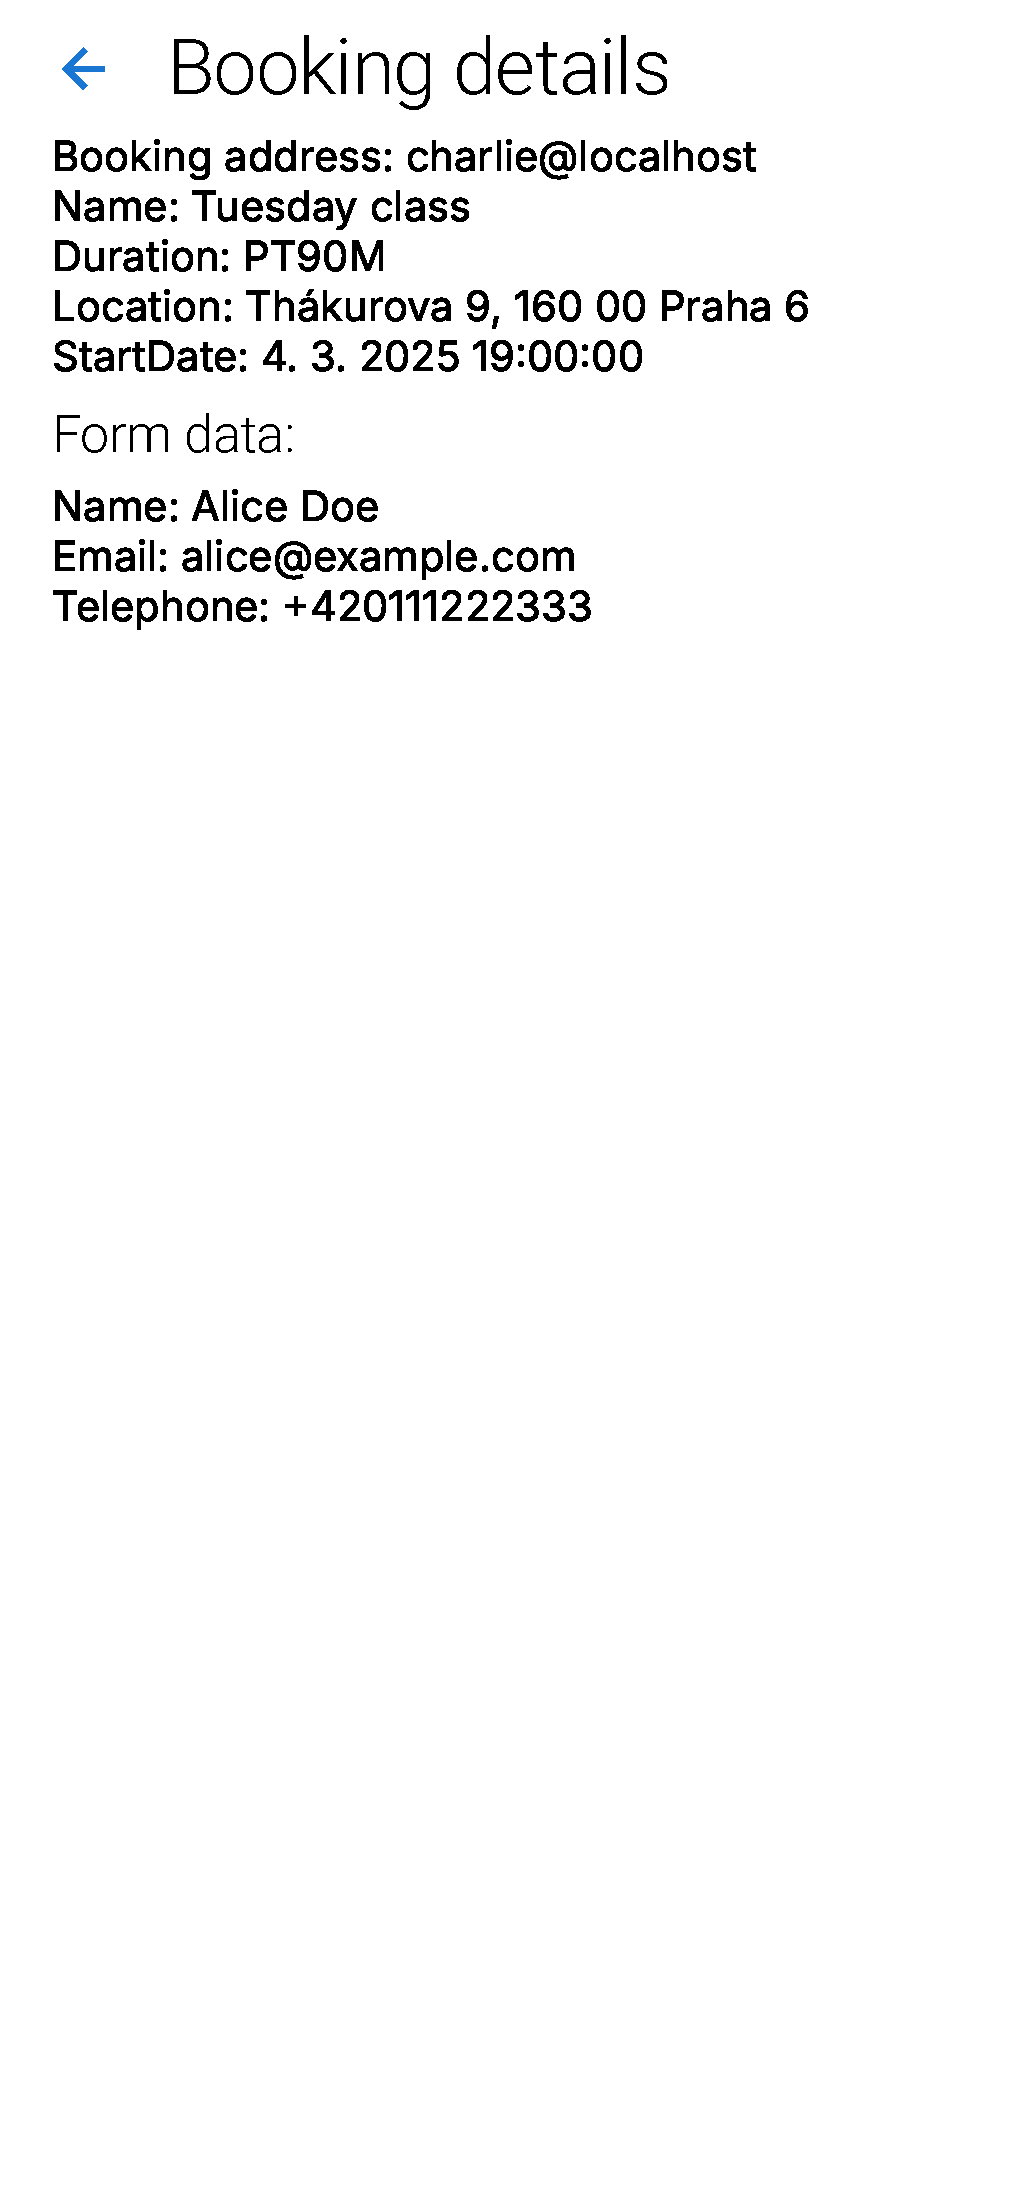
\includegraphics[width=0.48\textwidth]{content/implementation/client_app_home_booking_details.pdf}}
    \caption[Home page -- Item booking detail]{Home page in the item booking detail state}
    \label{fig:home_page_booking_details}
\end{figure}

\subsubsection{New booking}

The new booking page, available under the path \mintinline{text}{/book}, contains a form similar to the one for creating a new booking address. Here, the user inputs an entire booking address (rather than only a username). After filling in the booking address (which is again validated as the user types) and clicking on the \enquote{see inventory} button at the bottom-right of the page, the user is redirected to an items for booking page. At the top, there is also a title of the page along with a back button that redirects the user to the home page. The new booking page can be seen in the figure~\ref{fig:new_booking_page}.

\begin{figure}
    \centering
    \fbox{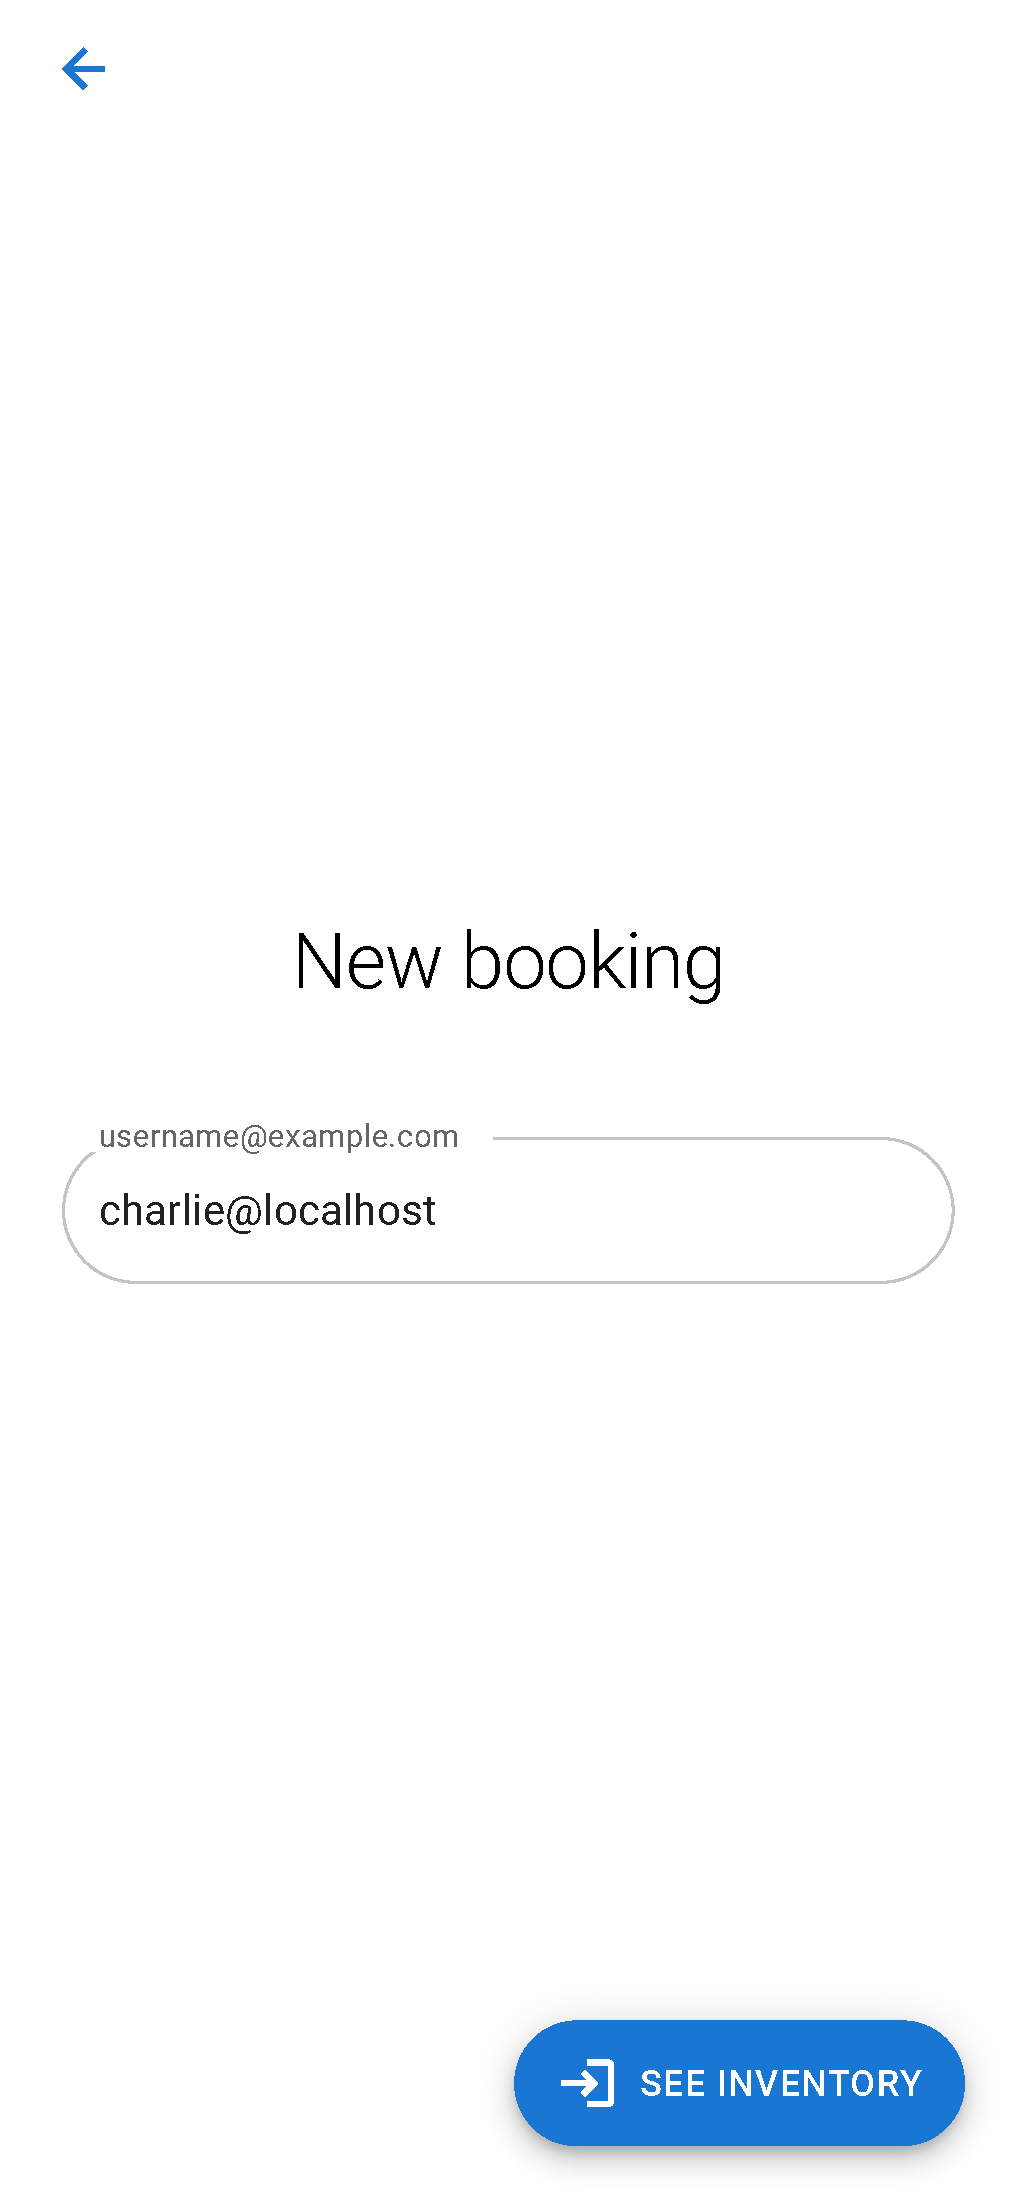
\includegraphics[width=0.48\textwidth]{content/implementation/client_app_new_booking.pdf}}
    \caption[New booking page]{New booking page}
    \label{fig:new_booking_page}
\end{figure}

\subsubsection{Items for booking}

The items for booking page, presented in the figure~\ref{fig:items_for_booking_page}, available under the path \mintinline{text}{/book/[address]}, where \mintinline{text}{[address]} is the URI-encoded booking address, whose inventory is to be fetched and displayed. Additionally, \mintinline{text}{[address]} can be an entire URI-encoded booking URL, which is used when opening an installed booking client PWA application using a booking URL such as \mintinline{text}{web+booking://username~example.com}, under supported platforms.

After the page is opened, the inventory of the requested booking address is fetched and in case of an error, an alert is displayed to the user. Then, the page displays the inventory details and metadata, and the items available for booking, along with a snippet of their metadata and occupancy. When the user clicks and item, the page switches to a second state, showing item details. As with the previous page, there is a header with the page title and a button to go back to the home page.

\begin{figure}
    \centering
    \fbox{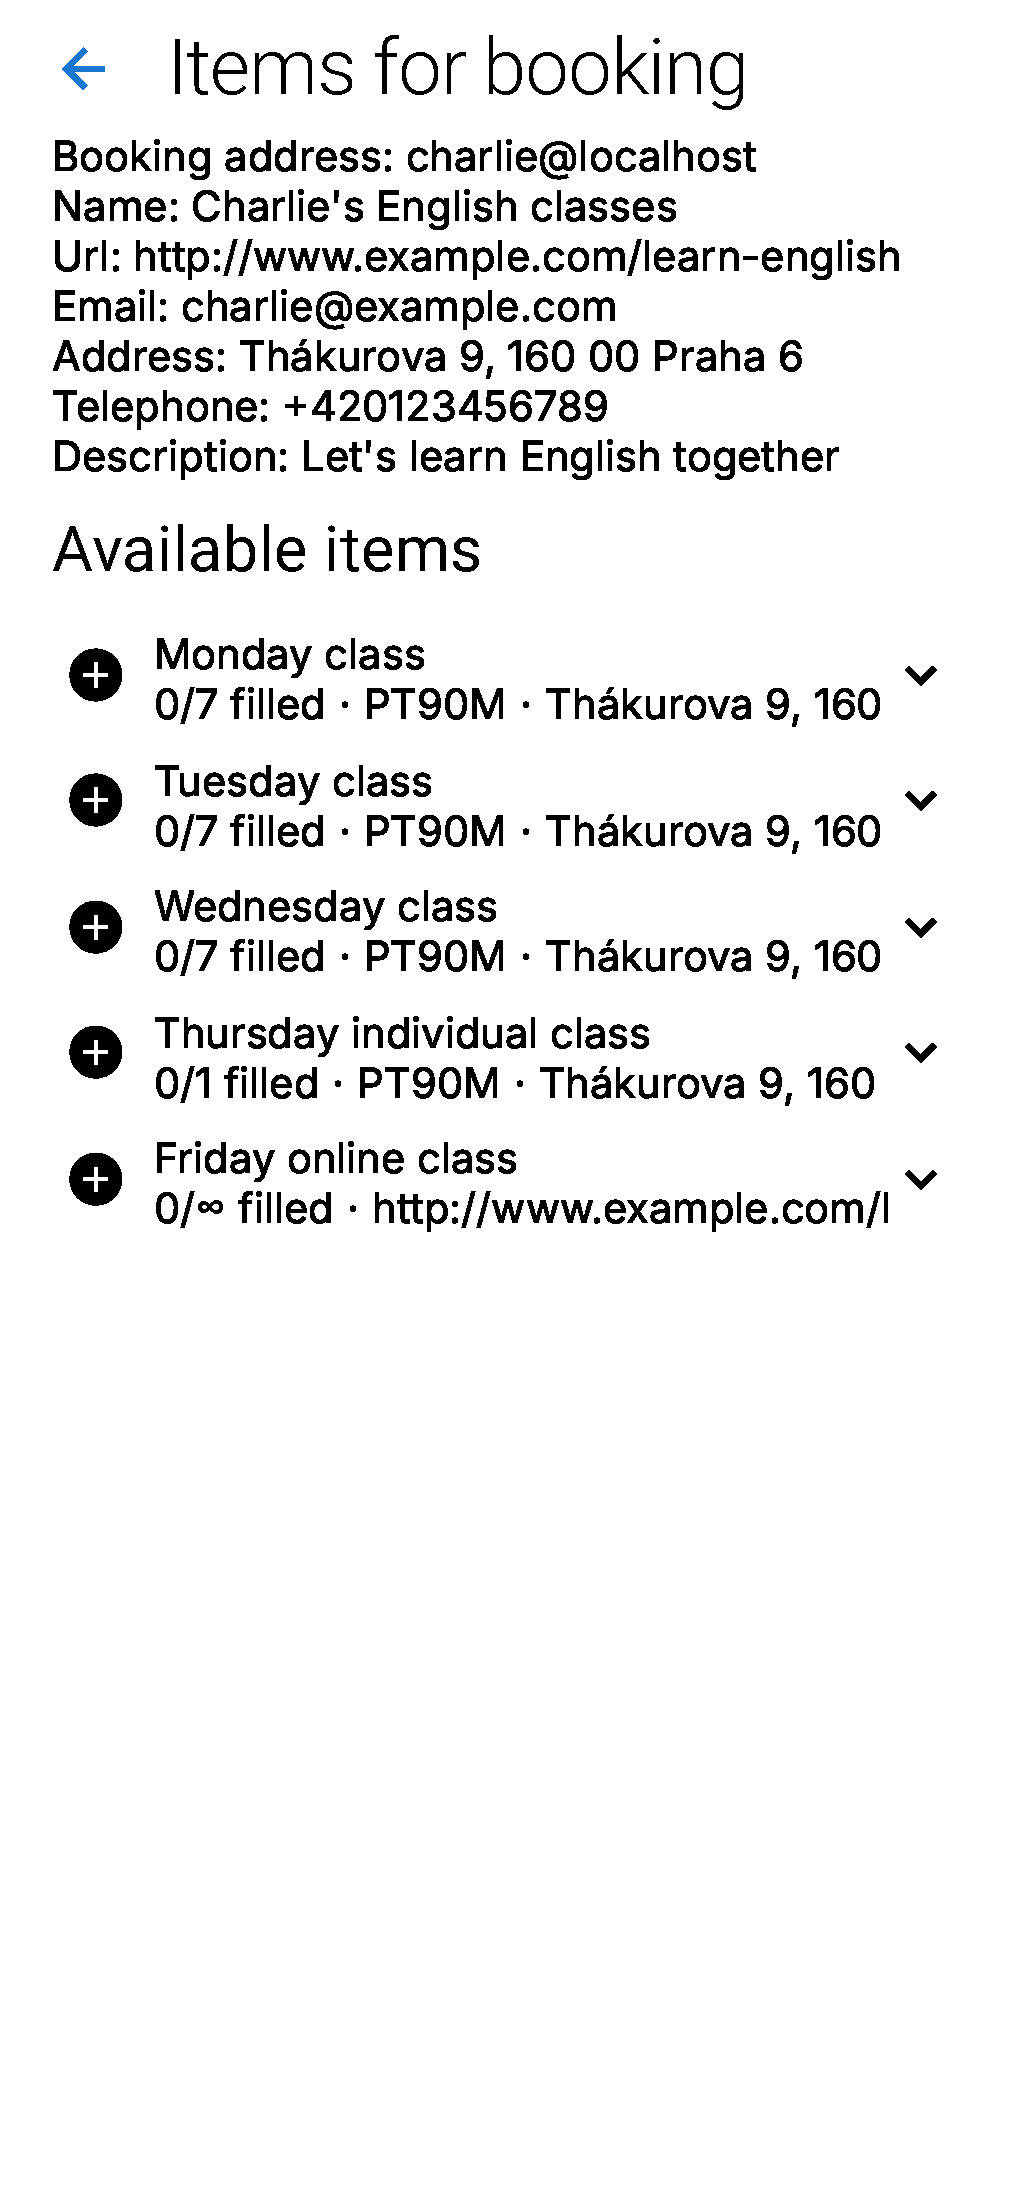
\includegraphics[width=0.48\textwidth]{content/implementation/client_app_new_booking_items.pdf}}
    \caption[Items for booking page]{Items for booking page with the requested booking address inventory and its items}
    \label{fig:items_for_booking_page}
\end{figure}

In the item details state, the page first shows the item data and metadata, followed by a booking form for the user to fill out. The booking form is generated dynamically, based on the JSON Schema present in the item data. This is done using the JSON Forms library. There is also a header with a title and a button to go back to the basic items for booking state. After the user fills out the form and clicks the \enquote{create booking} button on the bottom-right, a request for booking the selected items with the filled-out form attached is sent (first through the API gateway to the user's own booking service, then from the user's booking service to the item inventory's owner's booking service). If there has been an error in the process, an alert is shown, otherwise, the user is redirected to the home page. Item details with a filled-out form, along with an alert after unsuccessful booking, can be seen in the figure~\ref{fig:items_for_booking_page_item_details}. This, along with the home page, fulfills functional requirement~\ref{req:booking}.

\begin{figure}
    \centering
    \fbox{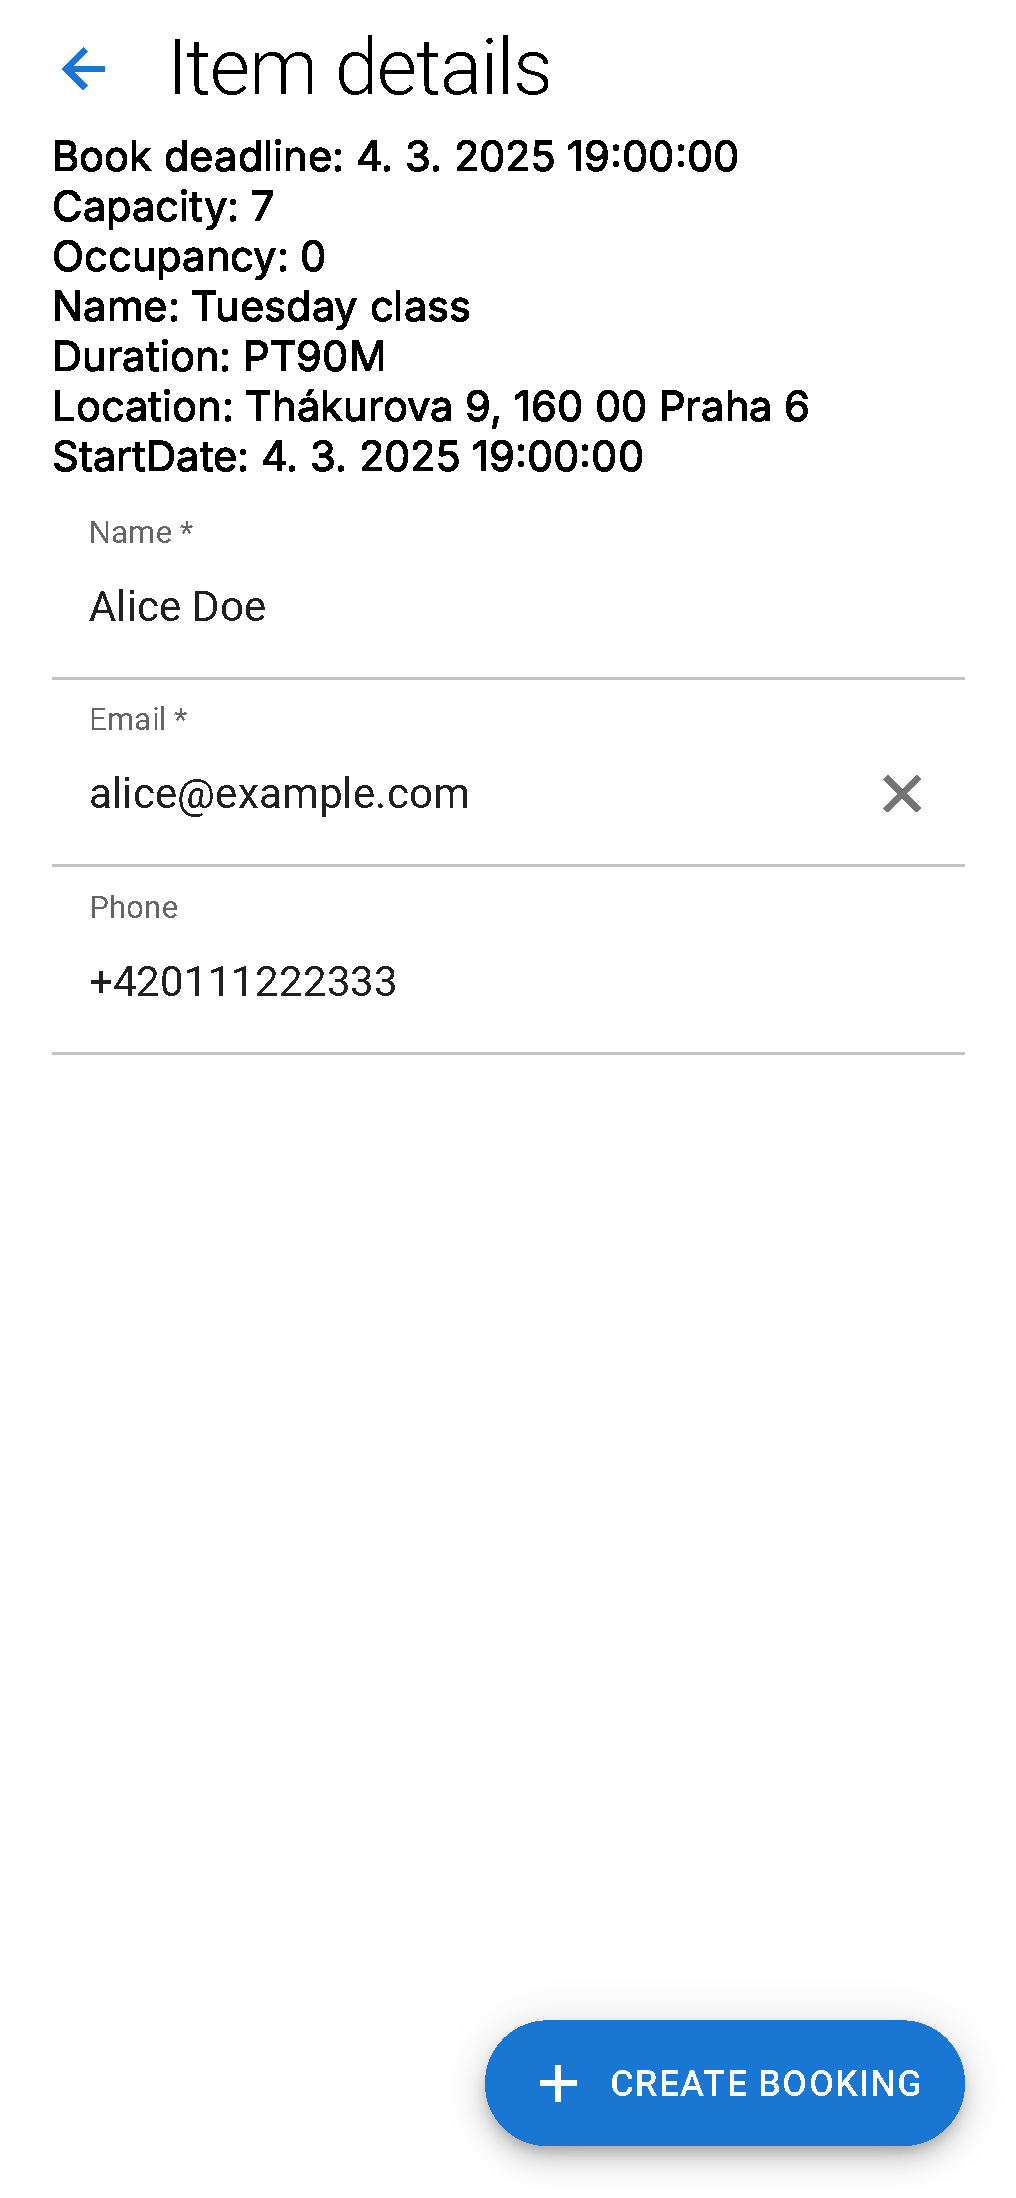
\includegraphics[width=0.48\textwidth]{content/implementation/client_app_new_booking_item_details_filled.pdf}}
    \hfill
    \fbox{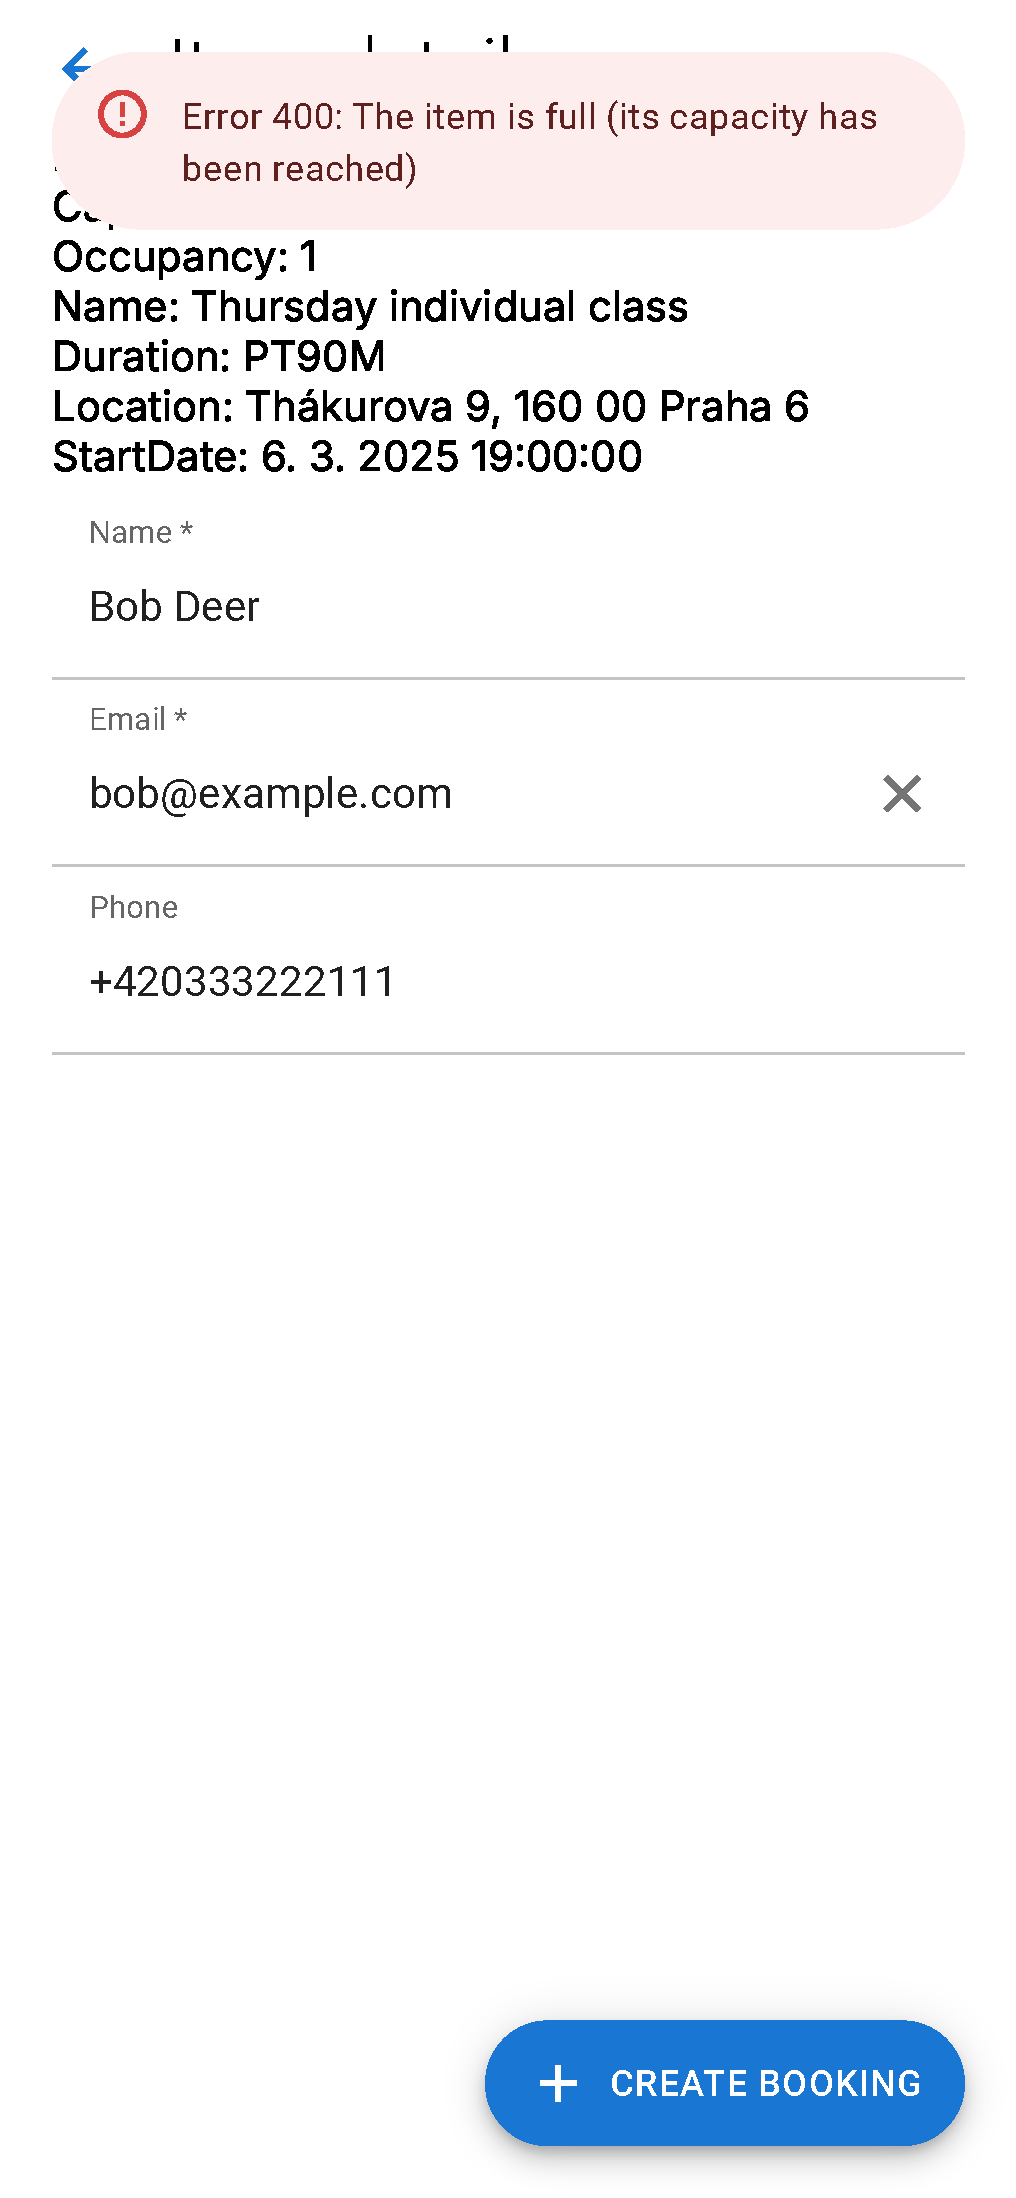
\includegraphics[width=0.48\textwidth]{content/implementation/client_app_new_booking_item_details_error_fully_booked.pdf}}
    \caption[Items for booking page -- Item details]{Item details state of the items for booking page, showing item information, metadata, and filled-out form to the left, and an alert upon unsuccessful booking to the right}
    \label{fig:items_for_booking_page_item_details}
\end{figure}

\subsubsection{Business}

The business page, shown in the figure~\ref{fig:items_for_booking_page_item_details} and available under the path \mintinline{text}{/business}, has two main states, create an inventory, and view inventory items.

The create an inventory state is used when a user has no inventory. The user is then presented a form to fill out inventory details and metadata. This form is dynamically generated using the JSON Forms library from a JSON Schema, but the JSON Schema is currently static for the entire client application based on the designed use case. In the future, there could be multiple pre-defined schemas for different use cases, as well as, for instance, an option to upload a custom schema. When the user fills out the form and submits using the \enquote{create} button at the bottom-right of the page and confirms a dialog that pops out, their inventory is created and they become a bookable user.

The view inventory items state is shown to bookable users. It contains a list of the items in the user's inventory, including snippets of the item's information (such as occupancy) and metadata. Upon clicking an item from the list, the user is redirected to the inventory item detail page. There is also a \enquote{add item} button at the bottom-right of the page, which redirects the user to the add item page.

Both states of this page share a menubar at the top of the page, which works analogically to the one on the home page.

\begin{figure}
    \centering
    \fbox{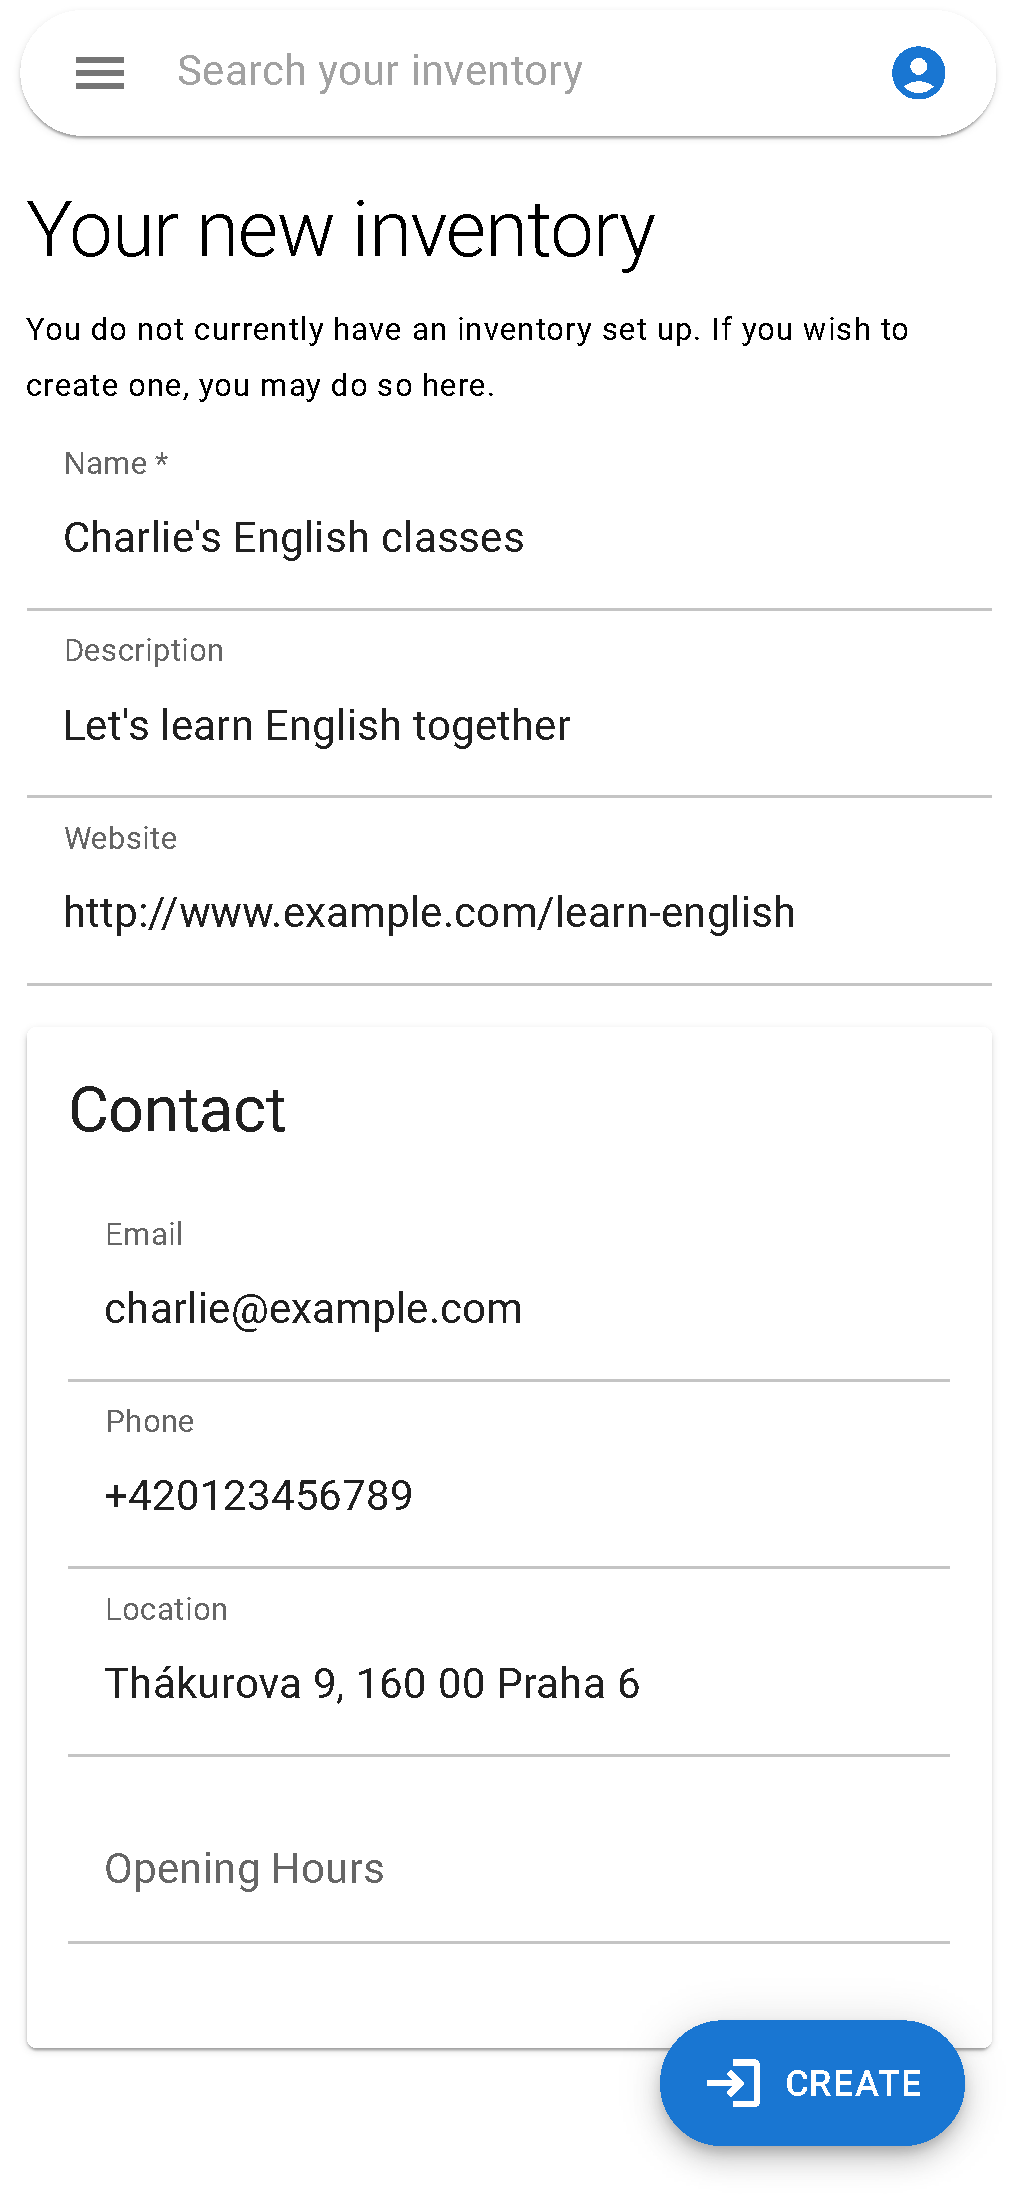
\includegraphics[width=0.48\textwidth]{content/implementation/client_app_business_create_inventory_filled.pdf}}
    \hfill
    \fbox{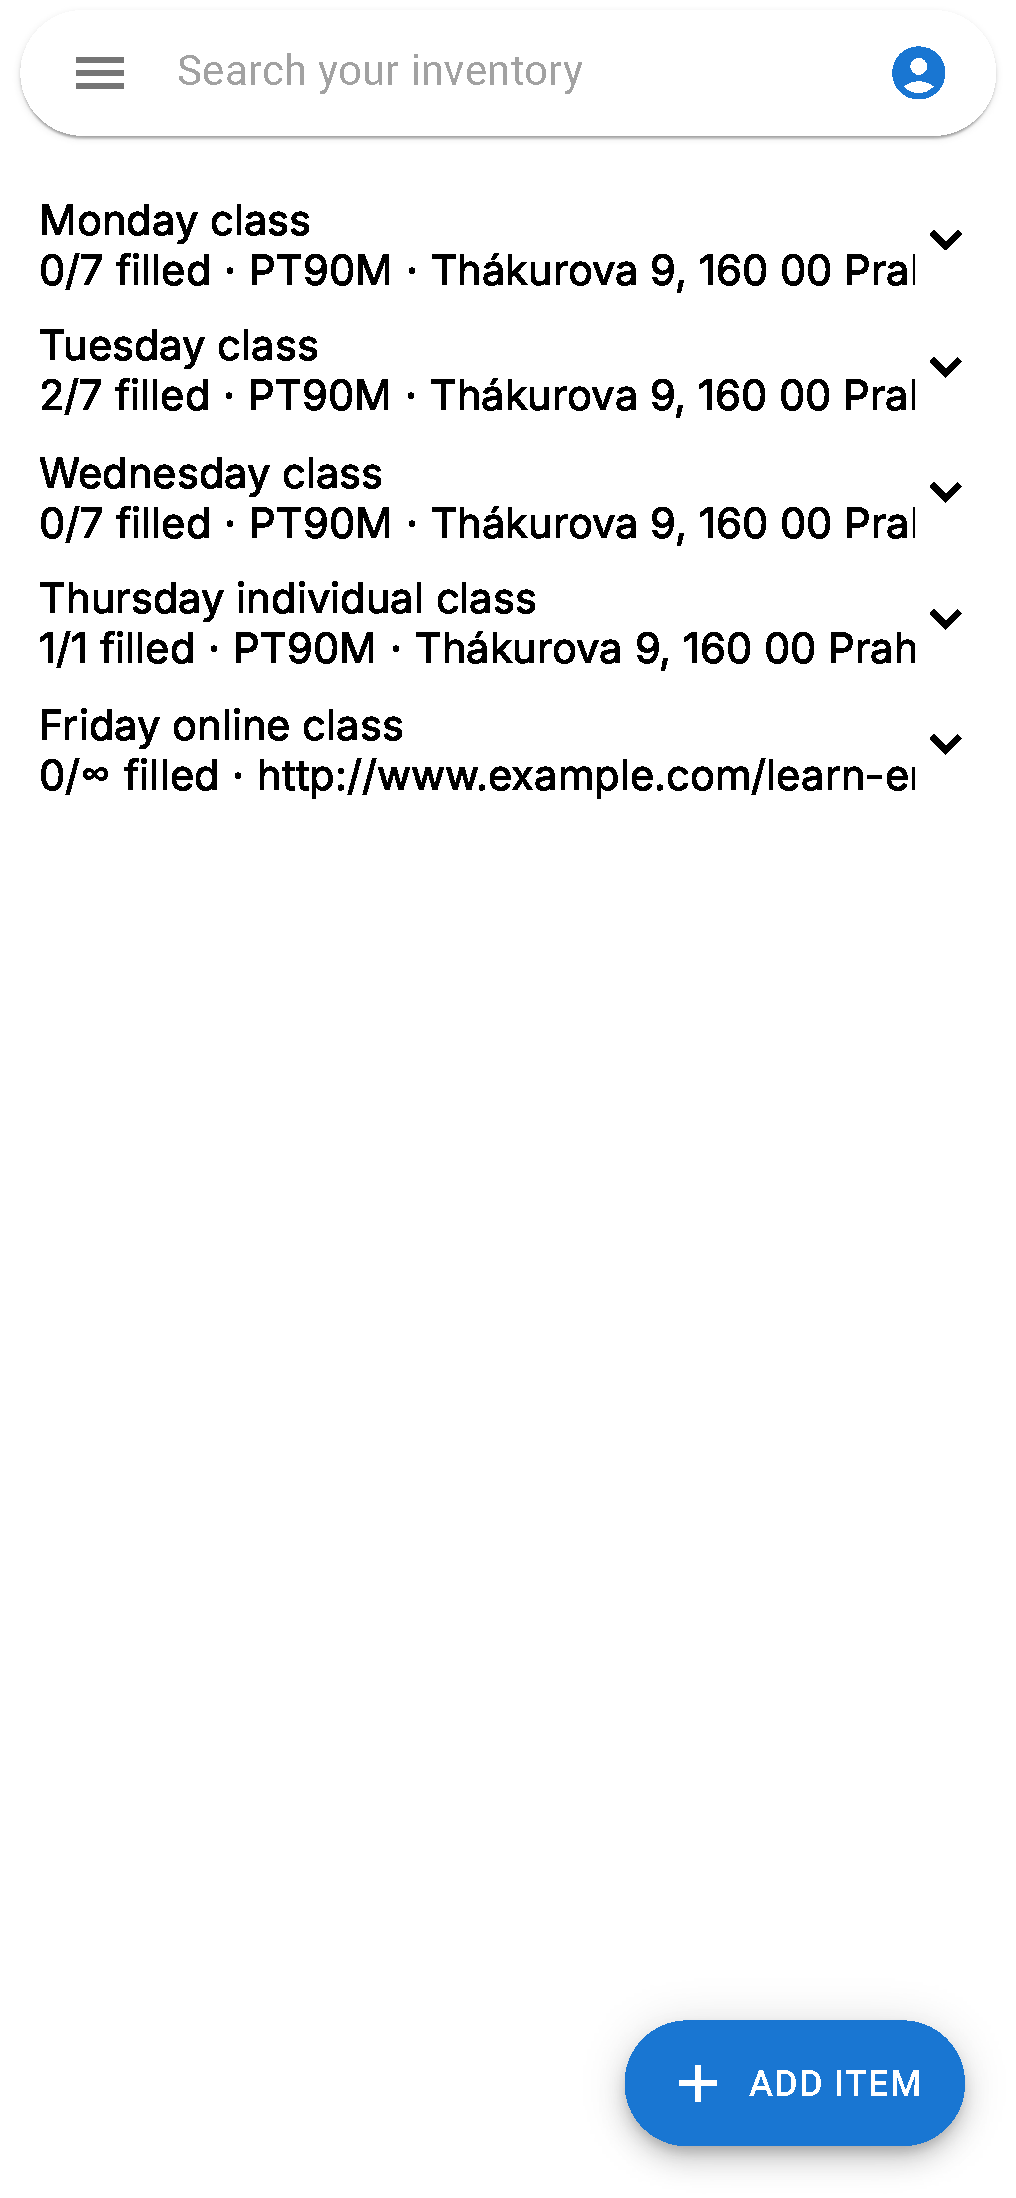
\includegraphics[width=0.48\textwidth]{content/implementation/client_app_business_inventory.pdf}}
    \caption[Business page]{Business page in the create new inventory state seen left, business page with a list of inventory items to the right}
    \label{fig:items_for_booking_page_item_details}
\end{figure}

\subsubsection{Add item page}

The add item page, available under the path \mintinline{text}{/business/add-item}, features a dynamically generated form, that the bookable user uses to fill out item information and metadata. As with the inventory creation form, the JSON Schema used is currently static for the client application, but adding new ones in the future should be simple. After filling out the form, the user clicks the \enquote{add} button, confirm a dialog and creates a new item. In case of an error during the item creation, an alert is shown. After successful item creation, the user is redirected back to the business page. The page is displayed in the figure~\ref{fig:add_item_page}. This, together with the business page, fulfills functional requirements~\ref{req:inventory} and~\ref{req:forms}. Moreover, together with the booking pages and mechanisms, it fulfills functional requirement~\ref{req:deadlines}.

\begin{figure}
    \centering
    \fbox{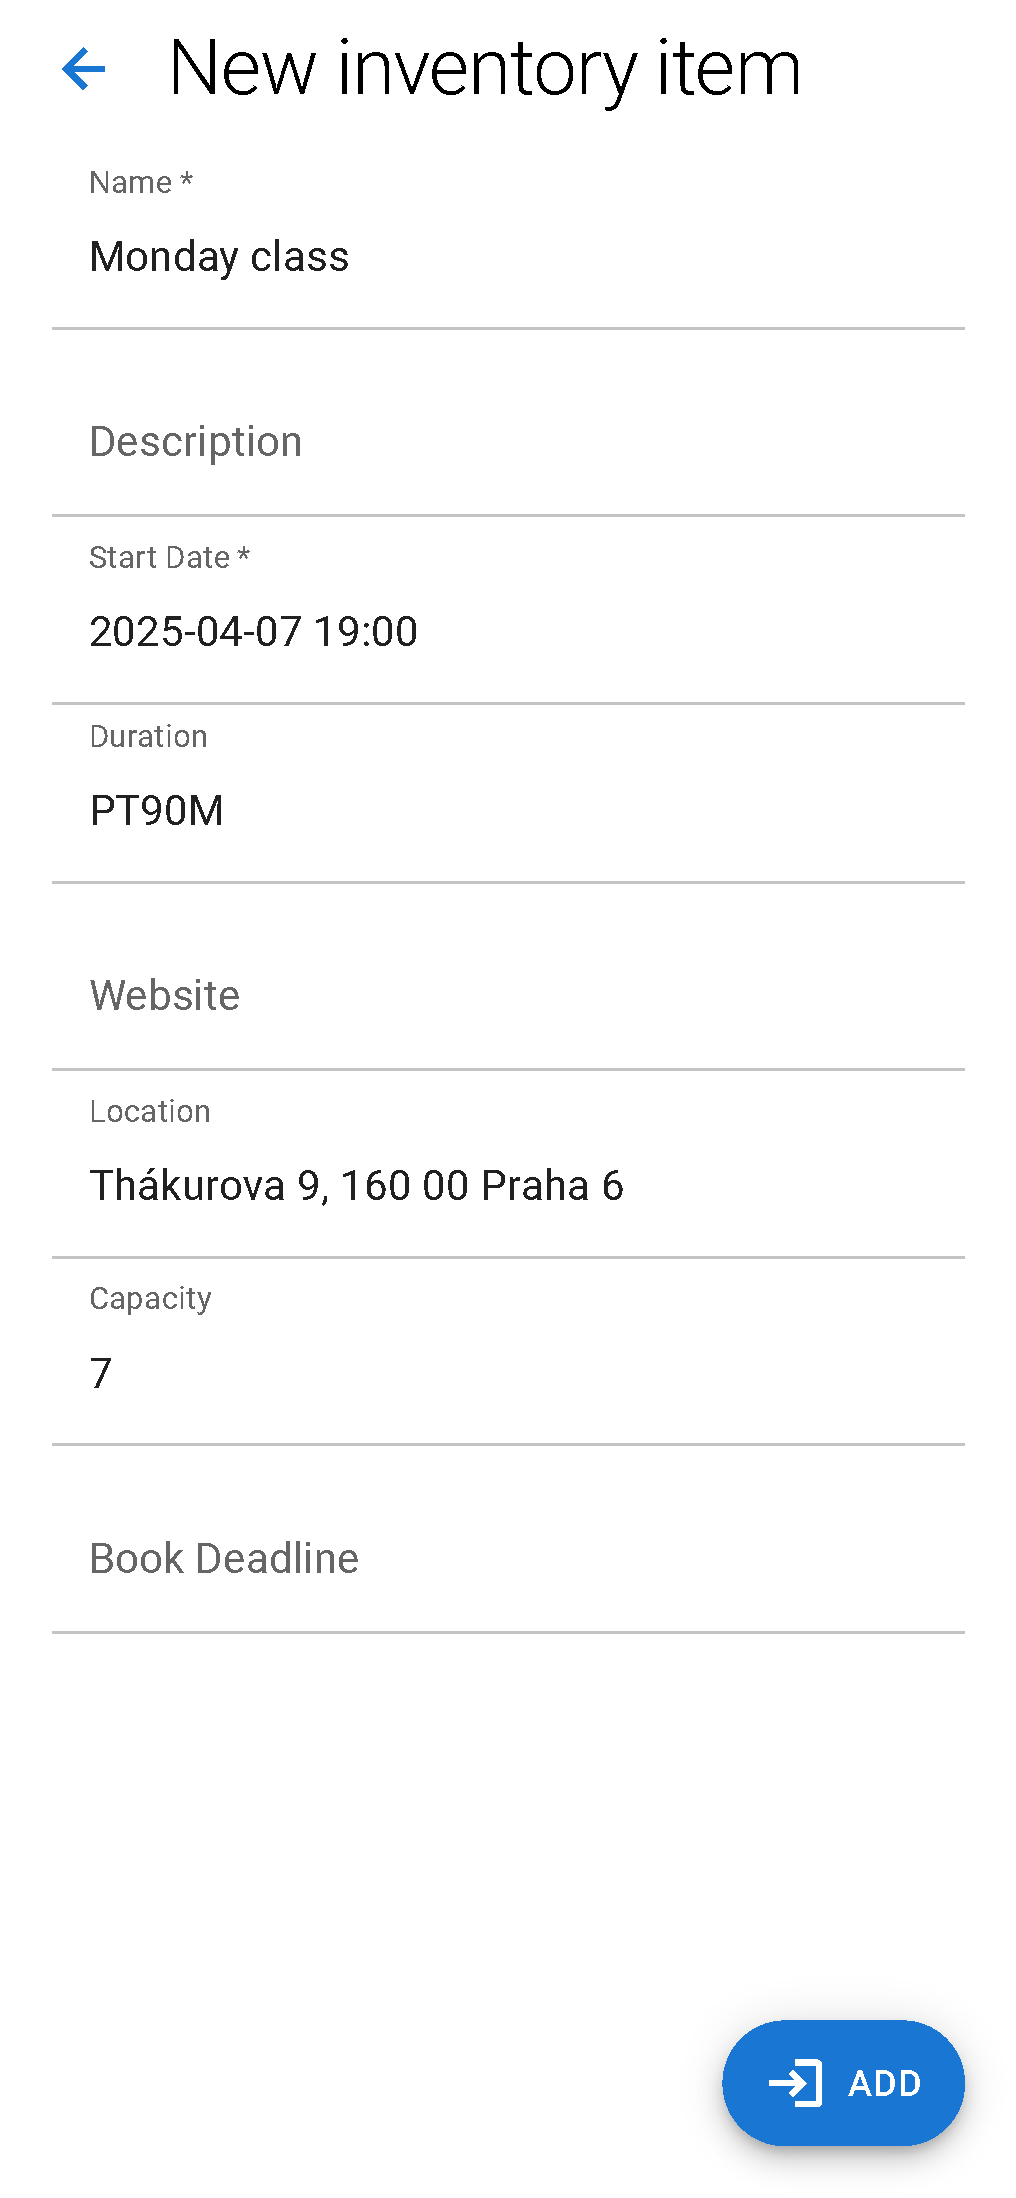
\includegraphics[width=0.48\textwidth]{content/implementation/client_app_business_inventory_add_item_filled.pdf}}
    \caption[Add item page]{Add item page}
    \label{fig:add_item_page}
\end{figure}

\subsubsection{Inventory item detail page}

\begin{sloppypar}
The inventory item detail page, available under the path \mintinline{text}{/business/items/[itemId]}, where \mintinline{text}{[itemId]} is the id of the item that should be shown, has two main states. Its first state -- item details -- shows information about the selected item along with a list of its bookings and snippets of the bookings' information. After clicking on a booking, the page switches to its second state, where the user is shown details of the selected booking, including its form data. Both states feature a page heading at the top, along with a button to go back to the business page, respectively to the item detail state in the case. The page can be seen in the figure~\ref{fig:inventory_item_detail_page}.
\end{sloppypar}

\begin{figure}
    \centering
    \fbox{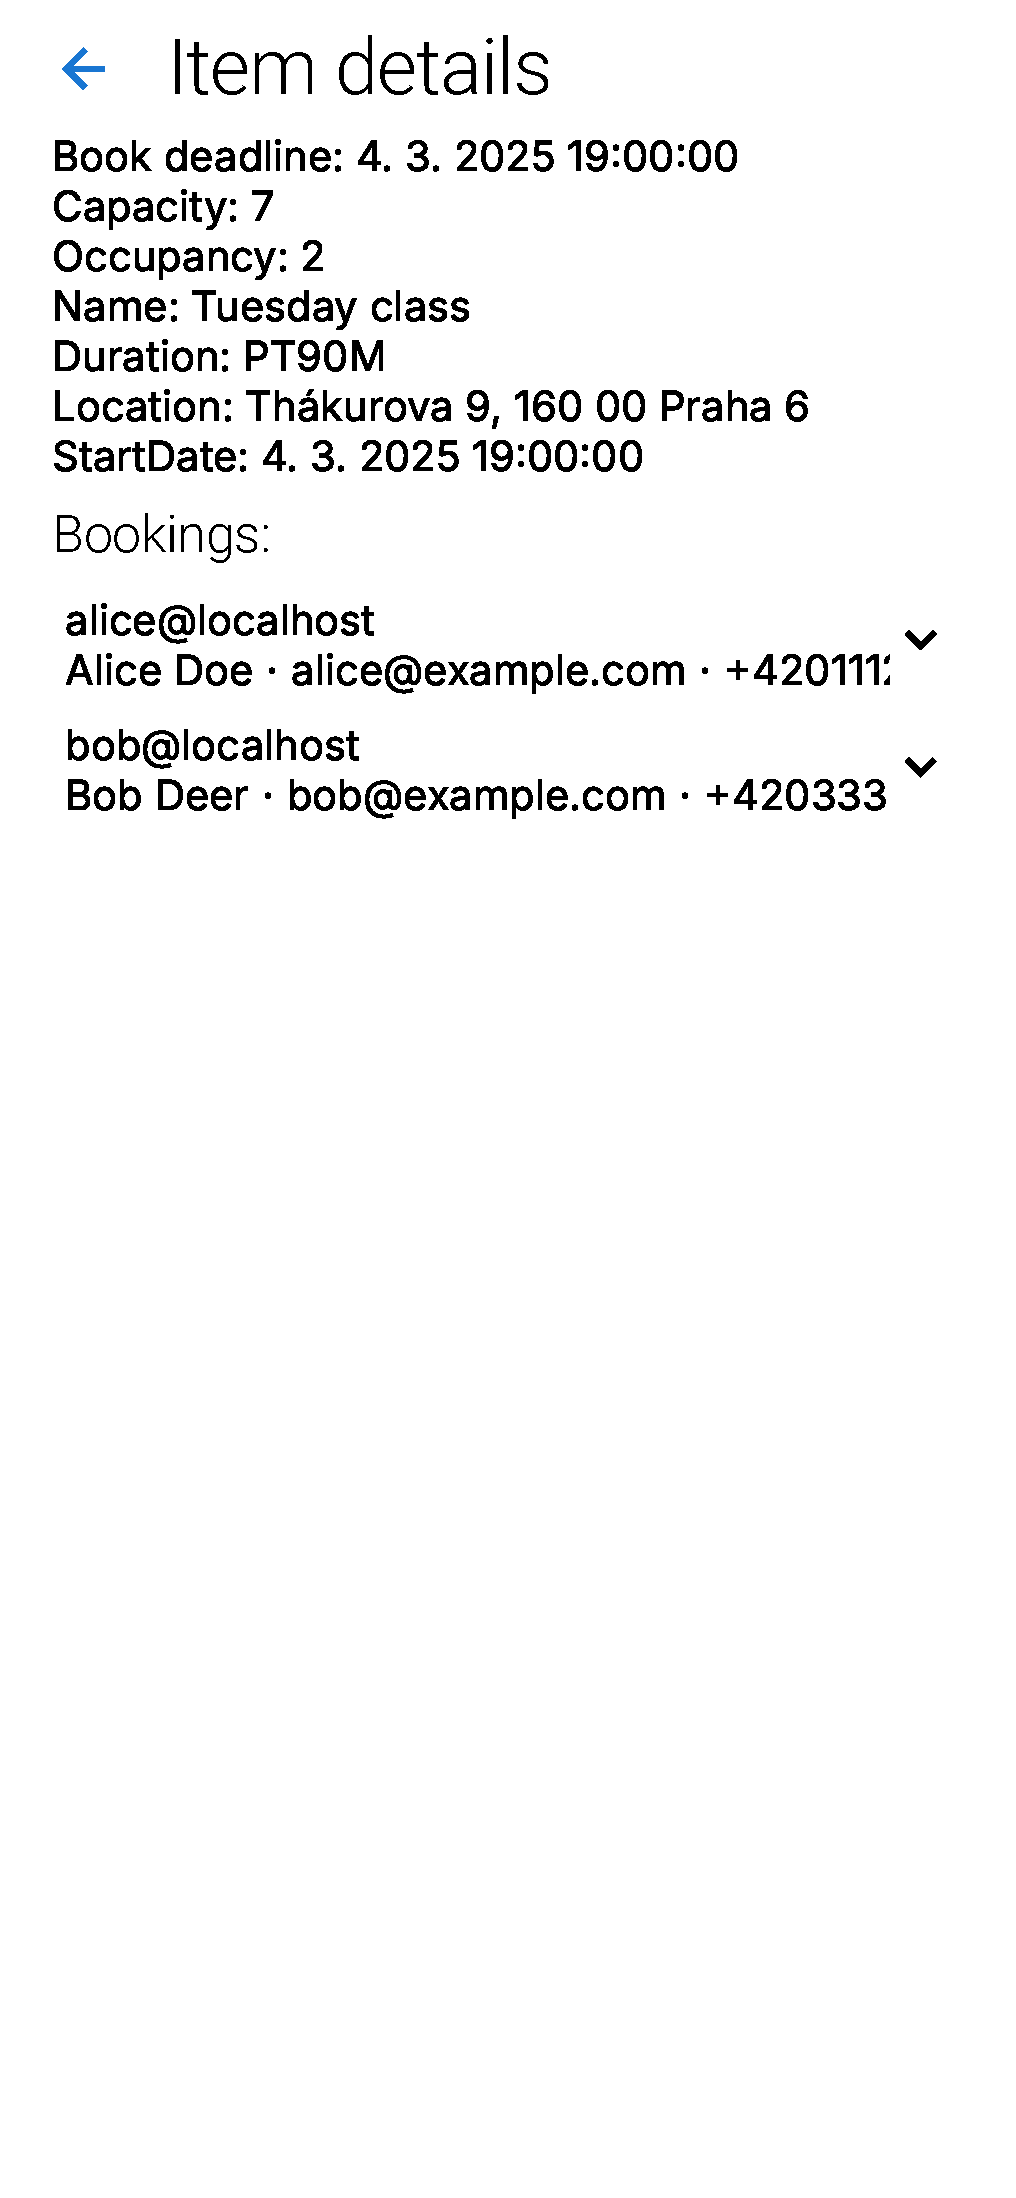
\includegraphics[width=0.48\textwidth]{content/implementation/client_app_business_inventory_item_details_bookings.pdf}}
    \hfill
    \fbox{
\includegraphics[width=0.48\textwidth]{content/implementation/client_app_business_inventory_item_booking_details.pdf}}
    \caption[Inventory item detail page]{Inventory item detail page, with its item detail state to the left, and booking detail to the right}
    \label{fig:inventory_item_detail_page}
\end{figure}
